\documentclass[oneside,a4paper,11pt]{book}
\usepackage[margin=1in]{geometry}

\usepackage{graphicx}
\usepackage[utf8]{inputenc} % allow utf-8 input
\usepackage[T1]{fontenc}    % use 8-bit T1 fonts
\usepackage{hyperref}       % hyperlinks
\usepackage{url}            % simple URL typesetting
\usepackage{booktabs}       % professional-quality tables
\usepackage{listings}
\usepackage{nicefrac}       % compact symbols for 1/2, etc.
\usepackage{xcolor}
\definecolor{codegreen}{rgb}{0,0.6,0}
\definecolor{codegray}{rgb}{0.5,0.5,0.5}
\definecolor{codepurple}{rgb}{0.58,0,0.82}
\definecolor{backcolour}{rgb}{0.95,0.95,0.92}

\lstdefinestyle{mystyle}{
    backgroundcolor=\color{backcolour},
    commentstyle=\color{codegreen},
    keywordstyle=\color{magenta},
    numberstyle=\tiny\color{codegray},
    stringstyle=\color{codepurple},
    basicstyle=\ttfamily\footnotesize,
    breakatwhitespace=false,
    breaklines=true,
    captionpos=b,
    keepspaces=true,
    numbers=left,
    numbersep=5pt,
    showspaces=false,
    showstringspaces=false,
    showtabs=false,
    tabsize=2
}
\lstset{style=mystyle}

\usepackage{microtype}      % microtypography

\usepackage[autostyle]{csquotes}
\usepackage{dsfont}

%\usepackage{algorithm,algpseudocode}
\usepackage[ruled,vlined]{algorithm2e}
\usepackage{multicol}

\usepackage{hyperref}
\usepackage[toc,title]{appendix}

\setlength{\parindent}{0pt}
\setlength{\parskip}{1em}

\newtheorem{theorem}{Theorem}
\newtheorem{definition}{Definition}
\newtheorem{proposition}{Proposition}
\newtheorem{corollary}{Corollary}

%\newcommand\scalemath[2]{\scalebox{#1}{\mbox{\ensuremath{\displaystyle #2}}}}


%%%%% NEW MATH DEFINITIONS %%%%%
\usepackage{amsmath,amsfonts,bm}
\usepackage{xspace}
\usepackage[nameinlink]{cleveref}


\crefformat{section}{\S#2#1#3} % see manual of cleveref, section 8.2.1
\crefname{algorithm}{Alg.}{Algs.}
\crefformat{subsection}{\S#2#1#3}
\Crefname{equation}{Eq.}{Eqs.}
\Crefname{figure}{Fig.}{Figs.}

%% abbr 
\newcommand{\ie}{{\em i.e.,}\xspace}
\newcommand{\cf}{{\em c.f.,}\xspace}
\newcommand{\eg}{{\em e.g.,}\xspace}
\newcommand{\etal}{{\em et al.,}\xspace}
\newcommand{\wrt}{\emph{w.r.t.}\xspace}
\newcommand{\aka}{\emph{a.k.a.}\xspace}
\newcommand{\resp}{\emph{resp.}\xspace}


\newcommand{\pos}{${pos}$}


%%% inline lists
\newcommand{\Ni}{({\em i})~}
\newcommand{\Nii}{({\em ii})~}
\newcommand{\Niii}{({\em iii})~}
\newcommand{\Niv}{({\em iv})~}
\newcommand{\Nv}{({\em v})~}
\newcommand{\Na}{({\em a})~}
\newcommand{\Nb}{({\em b})~}
\newcommand{\Nc}{({\em c})~}
\newcommand{\Nd}{({\em d})~}
\newcommand{\Ne}{({\em e})~}
\newcommand{\Nf}{({\em f})~}


\newcommand{\comm}[1]{\textcolor{blue}{\noindent #1}}
\newcommand{\alert}[1]{\textcolor{red}{\noindent$\Rightarrow$ #1}}
\newcommand{\red}[1]{\textcolor{red}{#1}}
\newcommand{\blue}[1]{\textcolor{blue}{#1}}
\newcommand{\magenta}[1]{\textcolor{magenta}{#1}}
\newcommand{\green}[1]{\textcolor{green}{#1}}
\newcommand{\teal}[1]{\textcolor{teal}{#1}}
\newcommand{\add}[1]{\textcolor{black}{#1}}

%\usepackage{amsmath,amsfonts,bm}
%\usepackage[tbtags]{amsmath}

% Mark sections of captions for referring to divisions of figures
\newcommand{\figleft}{{\em (Left)}}
\newcommand{\figcenter}{{\em (Center)}}
\newcommand{\figright}{{\em (Right)}}
\newcommand{\figtop}{{\em (Top)}}
\newcommand{\figbottom}{{\em (Bottom)}}
\newcommand{\captiona}{{\em (a)}}
\newcommand{\captionb}{{\em (b)}}
\newcommand{\captionc}{{\em (c)}}
\newcommand{\captiond}{{\em (d)}}


\newtheorem{prop}{Proposition}

\newcommand{\sarrow}[1][4pt]{\!\mathrel{%
   \vcenter{\hbox{\rule[-.5\fontdimen8\textfont3]{#1}{\fontdimen8\textfont3}}}%
   \mkern-4mu\hbox{\usefont{U}{lasy}{m}{n}\symbol{41}}}\!}
\makeatletter   
\newcommand{\sveryshortarrow}[1][3pt]{\mathrel{%
    \vcenter{\hbox{\rule[-.5\fontdimen8\scriptfont3]
               {\scriptratio\dimexpr#1\relax}{\fontdimen8\scriptfont3}}}%
   \mkern-4mu\hbox{\let\f@size\sf@size\usefont{U}{lasy}{m}{n}\symbol{41}}}}
\makeatother

% \newcommand{\sarrow}{{\veryshortarrow}}

\newtheorem{defi}{Definition}

% Highlight a newly defined term
\newcommand{\newterm}[1]{{\bf #1}}


% Figure reference, lower-case.
\def\figref#1{figure~\ref{#1}}
% Figure reference, capital. For start of sentence
\def\Figref#1{Figure~\ref{#1}}
\def\twofigref#1#2{figures \ref{#1} and \ref{#2}}
\def\quadfigref#1#2#3#4{figures \ref{#1}, \ref{#2}, \ref{#3} and \ref{#4}}
% Section reference, lower-case.
\def\secref#1{section~\ref{#1}}
% Section reference, capital.
\def\Secref#1{Section~\ref{#1}}
% Reference to two sections.
\def\twosecrefs#1#2{sections \ref{#1} and \ref{#2}}
% Reference to three sections.
\def\secrefs#1#2#3{sections \ref{#1}, \ref{#2} and \ref{#3}}
% Reference to an equation, lower-case.
\def\eqref#1{equation~\ref{#1}}
% Reference to an equation, upper case
\def\Eqref#1{Equation~\ref{#1}}
% A raw reference to an equation---avoid using if possible
\def\plaineqref#1{\ref{#1}}
% Reference to a chapter, lower-case.
\def\chapref#1{chapter~\ref{#1}}
% Reference to an equation, upper case.
\def\Chapref#1{Chapter~\ref{#1}}
% Reference to a range of chapters
\def\rangechapref#1#2{chapters\ref{#1}--\ref{#2}}
% Reference to an algorithm, lower-case.
\def\algref#1{algorithm~\ref{#1}}
% Reference to an algorithm, upper case.
\def\Algref#1{Algorithm~\ref{#1}}
\def\twoalgref#1#2{algorithms \ref{#1} and \ref{#2}}
\def\Twoalgref#1#2{Algorithms \ref{#1} and \ref{#2}}
% Reference to a part, lower case
\def\partref#1{part~\ref{#1}}
% Reference to a part, upper case
\def\Partref#1{Part~\ref{#1}}
\def\twopartref#1#2{parts \ref{#1} and \ref{#2}}

\def\ceil#1{\lceil #1 \rceil}
\def\floor#1{\lfloor #1 \rfloor}
\def\1{\bm{1}}
\newcommand{\train}{\mathcal{D}}
\newcommand{\valid}{\mathcal{D_{\mathrm{valid}}}}
\newcommand{\test}{\mathcal{D_{\mathrm{test}}}}

\def\eps{{\epsilon}}


% Random variables
\def\reta{{\textnormal{$\eta$}}}
\def\ra{{\textnormal{a}}}
\def\rb{{\textnormal{b}}}
\def\rc{{\textnormal{c}}}
\def\rd{{\textnormal{d}}}
\def\re{{\textnormal{e}}}
\def\rf{{\textnormal{f}}}
\def\rg{{\textnormal{g}}}
\def\rh{{\textnormal{h}}}
\def\ri{{\textnormal{i}}}
\def\rj{{\textnormal{j}}}
\def\rk{{\textnormal{k}}}
\def\rl{{\textnormal{l}}}
% rm is already a command, just don't name any random variables m
\def\rn{{\textnormal{n}}}
\def\ro{{\textnormal{o}}}
\def\rp{{\textnormal{p}}}
\def\rq{{\textnormal{q}}}
\def\rr{{\textnormal{r}}}
\def\rs{{\textnormal{s}}}
\def\rt{{\textnormal{t}}}
\def\ru{{\textnormal{u}}}
\def\rv{{\textnormal{v}}}
\def\rw{{\textnormal{w}}}
\def\rx{{\textnormal{x}}}
\def\ry{{\textnormal{y}}}
\def\rz{{\textnormal{z}}}

% Random vectors
\def\rvepsilon{{\mathbf{\epsilon}}}
\def\rvtheta{{\mathbf{\theta}}}
\def\rva{{\mathbf{a}}}
\def\rvb{{\mathbf{b}}}
\def\rvc{{\mathbf{c}}}
\def\rvd{{\mathbf{d}}}
\def\rve{{\mathbf{e}}}
\def\rvf{{\mathbf{f}}}
\def\rvg{{\mathbf{g}}}
\def\rvh{{\mathbf{h}}}
\def\rvu{{\mathbf{i}}}
\def\rvj{{\mathbf{j}}}
\def\rvk{{\mathbf{k}}}
\def\rvl{{\mathbf{l}}}
\def\rvm{{\mathbf{m}}}
\def\rvn{{\mathbf{n}}}
\def\rvo{{\mathbf{o}}}
\def\rvp{{\mathbf{p}}}
\def\rvq{{\mathbf{q}}}
\def\rvr{{\mathbf{r}}}
\def\rvs{{\mathbf{s}}}
\def\rvt{{\mathbf{t}}}
\def\rvu{{\mathbf{u}}}
\def\rvv{{\mathbf{v}}}
\def\rvw{{\mathbf{w}}}
\def\rvx{{\mathbf{x}}}
\def\rvy{{\mathbf{y}}}
\def\rvz{{\mathbf{z}}}

% Elements of random vectors
\def\erva{{\textnormal{a}}}
\def\ervb{{\textnormal{b}}}
\def\ervc{{\textnormal{c}}}
\def\ervd{{\textnormal{d}}}
\def\erve{{\textnormal{e}}}
\def\ervf{{\textnormal{f}}}
\def\ervg{{\textnormal{g}}}
\def\ervh{{\textnormal{h}}}
\def\ervi{{\textnormal{i}}}
\def\ervj{{\textnormal{j}}}
\def\ervk{{\textnormal{k}}}
\def\ervl{{\textnormal{l}}}
\def\ervm{{\textnormal{m}}}
\def\ervn{{\textnormal{n}}}
\def\ervo{{\textnormal{o}}}
\def\ervp{{\textnormal{p}}}
\def\ervq{{\textnormal{q}}}
\def\ervr{{\textnormal{r}}}
\def\ervs{{\textnormal{s}}}
\def\ervt{{\textnormal{t}}}
\def\ervu{{\textnormal{u}}}
\def\ervv{{\textnormal{v}}}
\def\ervw{{\textnormal{w}}}
\def\ervx{{\textnormal{x}}}
\def\ervy{{\textnormal{y}}}
\def\ervz{{\textnormal{z}}}

% Random matrices
\def\rmA{{\mathbf{A}}}
\def\rmB{{\mathbf{B}}}
\def\rmC{{\mathbf{C}}}
\def\rmD{{\mathbf{D}}}
\def\rmE{{\mathbf{E}}}
\def\rmF{{\mathbf{F}}}
\def\rmG{{\mathbf{G}}}
\def\rmH{{\mathbf{H}}}
\def\rmI{{\mathbf{I}}}
\def\rmJ{{\mathbf{J}}}
\def\rmK{{\mathbf{K}}}
\def\rmL{{\mathbf{L}}}
\def\rmM{{\mathbf{M}}}
\def\rmN{{\mathbf{N}}}
\def\rmO{{\mathbf{O}}}
\def\rmP{{\mathbf{P}}}
\def\rmQ{{\mathbf{Q}}}
\def\rmR{{\mathbf{R}}}
\def\rmS{{\mathbf{S}}}
\def\rmT{{\mathbf{T}}}
\def\rmU{{\mathbf{U}}}
\def\rmV{{\mathbf{V}}}
\def\rmW{{\mathbf{W}}}
\def\rmX{{\mathbf{X}}}
\def\rmY{{\mathbf{Y}}}
\def\rmZ{{\mathbf{Z}}}

% Elements of random matrices
\def\ermA{{\textnormal{A}}}
\def\ermB{{\textnormal{B}}}
\def\ermC{{\textnormal{C}}}
\def\ermD{{\textnormal{D}}}
\def\ermE{{\textnormal{E}}}
\def\ermF{{\textnormal{F}}}
\def\ermG{{\textnormal{G}}}
\def\ermH{{\textnormal{H}}}
\def\ermI{{\textnormal{I}}}
\def\ermJ{{\textnormal{J}}}
\def\ermK{{\textnormal{K}}}
\def\ermL{{\textnormal{L}}}
\def\ermM{{\textnormal{M}}}
\def\ermN{{\textnormal{N}}}
\def\ermO{{\textnormal{O}}}
\def\ermP{{\textnormal{P}}}
\def\ermQ{{\textnormal{Q}}}
\def\ermR{{\textnormal{R}}}
\def\ermS{{\textnormal{S}}}
\def\ermT{{\textnormal{T}}}
\def\ermU{{\textnormal{U}}}
\def\ermV{{\textnormal{V}}}
\def\ermW{{\textnormal{W}}}
\def\ermX{{\textnormal{X}}}
\def\ermY{{\textnormal{Y}}}
\def\ermZ{{\textnormal{Z}}}

% Vectors
\def\vzero{{\bm{0}}}
\def\vone{{\bm{1}}}
\def\vmu{{\bm{\mu}}}
\def\vtheta{{\bm{\theta}}}
\def\va{{\bm{a}}}
\def\vb{{\bm{b}}}
\def\vc{{\bm{c}}}
\def\vd{{\bm{d}}}
\def\ve{{\bm{e}}}
\def\vf{{\bm{f}}}
\def\vg{{\bm{g}}}
\def\vh{{\bm{h}}}
\def\vi{{\bm{i}}}
\def\vj{{\bm{j}}}
\def\vk{{\bm{k}}}
\def\vl{{\bm{l}}}
\def\vm{{\bm{m}}}
\def\vn{{\bm{n}}}
\def\vo{{\bm{o}}}
\def\vp{{\bm{p}}}
\def\vq{{\bm{q}}}
\def\vr{{\bm{r}}}
\def\vs{{\bm{s}}}
\def\vt{{\bm{t}}}
\def\vu{{\bm{u}}}
\def\vv{{\bm{v}}}
\def\vw{{\bm{w}}}
\def\vx{{\bm{x}}}
\def\vy{{\bm{y}}}
\def\vz{{\bm{z}}}

\def\vip{{\bm{i}\bm{p}}}

\def\vdelta{{\bm{\delta}}}
\def\valphaa{{\bm{\alpha}}}

% Elements of vectors
\def\evalpha{{\alpha}}
\def\evbeta{{\beta}}
\def\evepsilon{{\epsilon}}
\def\evlambda{{\lambda}}
\def\evomega{{\omega}}
\def\evmu{{\mu}}
\def\evpsi{{\psi}}
\def\evsigma{{\sigma}}
\def\evtheta{{\theta}}
\def\eva{{a}}
\def\evb{{b}}
\def\evc{{c}}
\def\evd{{d}}
\def\eve{{e}}
\def\evf{{f}}
\def\evg{{g}}
\def\evh{{h}}
\def\evi{{i}}
\def\evj{{j}}
\def\evk{{k}}
\def\evl{{l}}
\def\evm{{m}}
\def\evn{{n}}
\def\evo{{o}}
\def\evp{{p}}
\def\evq{{q}}
\def\evr{{r}}
\def\evs{{s}}
\def\evt{{t}}
\def\evu{{u}}
\def\evv{{v}}
\def\evw{{w}}
\def\evx{{x}}
\def\evy{{y}}
\def\evz{{z}}

% Matrix
\def\m1{{\bm{1}}}
\def\mA{{\bm{A}}}
\def\mB{{\bm{B}}}
\def\mC{{\bm{C}}}
\def\mD{{\bm{D}}}
\def\mE{{\bm{E}}}
\def\mF{{\bm{F}}}
\def\mG{{\bm{G}}}
\def\mH{{\bm{H}}}
\def\mI{{\bm{I}}}
\def\mJ{{\bm{J}}}
\def\mK{{\bm{K}}}
\def\mL{{\bm{L}}}
\def\mM{{\bm{M}}}
\def\mN{{\bm{N}}}
\def\mO{{\bm{O}}}
\def\mP{{\bm{P}}}
\def\mQ{{\bm{Q}}}
\def\mR{{\bm{R}}}
\def\mS{{\bm{S}}}
\def\mT{{\bm{T}}}
\def\mU{{\bm{U}}}
\def\mV{{\bm{V}}}
\def\mW{{\bm{W}}}
\def\mX{{\bm{X}}}
\def\mY{{\bm{Y}}}
\def\mZ{{\bm{Z}}}
\def\mBeta{{\bm{\beta}}}
\def\mPhi{{\bm{\Phi}}}
\def\mLambda{{\bm{\Lambda}}}
\def\mSigma{{\bm{\Sigma}}}

% Tensor
\DeclareMathAlphabet{\mathsfit}{\encodingdefault}{\sfdefault}{m}{sl}
\SetMathAlphabet{\mathsfit}{bold}{\encodingdefault}{\sfdefault}{bx}{n}

\newcommand{\tens}[1]{\bm{\mathsfit{#1}}}


\def\tA{{\tens{A}}}
\def\tB{{\tens{B}}}
\def\tC{{\tens{C}}}
\def\tD{{\tens{D}}}
\def\tE{{\tens{E}}}
\def\tF{{\tens{F}}}
\def\tG{{\tens{G}}}
\def\tH{{\tens{H}}}
\def\tI{{\tens{I}}}
\def\tJ{{\tens{J}}}
\def\tK{{\tens{K}}}
\def\tL{{\tens{L}}}
\def\tM{{\tens{M}}}
\def\tN{{\tens{N}}}
\def\tO{{\tens{O}}}
\def\tP{{\tens{P}}}
\def\tQ{{\tens{Q}}}
\def\tR{{\tens{R}}}
\def\tS{{\tens{S}}}
\def\tT{{\tens{T}}}
\def\tU{{\tens{U}}}
\def\tV{{\tens{V}}}
\def\tW{{\tens{W}}}
\def\tX{{\tens{X}}}
\def\tY{{\tens{Y}}}
\def\tZ{{\tens{Z}}}


% Graph
\def\gA{{\mathcal{A}}}
\def\gB{{\mathcal{B}}}
\def\gC{{\mathcal{C}}}
\def\gD{{\mathcal{D}}}
\def\gE{{\mathcal{E}}}
\def\gF{{\mathcal{F}}}
\def\gG{{\mathcal{G}}}
\def\gH{{\mathcal{H}}}
\def\gI{{\mathcal{I}}}
\def\gJ{{\mathcal{J}}}
\def\gK{{\mathcal{K}}}
\def\gL{{\mathcal{L}}}
\def\gM{{\mathcal{M}}}
\def\gN{{\mathcal{N}}}
\def\gO{{\mathcal{O}}}
\def\gP{{\mathcal{P}}}
\def\gQ{{\mathcal{Q}}}
\def\gR{{\mathcal{R}}}
\def\gS{{\mathcal{S}}}
\def\gT{{\mathcal{T}}}
\def\gU{{\mathcal{U}}}
\def\gV{{\mathcal{V}}}
\def\gW{{\mathcal{W}}}
\def\gX{{\mathcal{X}}}
\def\gY{{\mathcal{Y}}}
\def\gZ{{\mathcal{Z}}}
\def\gSP{{\mathcal{S}\mathcal{P}}}
\def\gLS{{\mathcal{L}\mathcal{S}}}
\def\gLU{{\mathcal{L}\mathcal{U}}}
\def\gST{{\mathcal{S}\mathcal{T}}}

% Sets
\def\sA{{\mathbb{A}}}
\def\sB{{\mathbb{B}}}
\def\sC{{\mathbb{C}}}
\def\sD{{\mathbb{D}}}
% Don't use a set called E, because this would be the same as our symbol
% for expectation.
\def\sF{{\mathbb{F}}}
\def\sG{{\mathbb{G}}}
\def\sH{{\mathbb{H}}}
\def\sI{{\mathbb{I}}}
\def\sJ{{\mathbb{J}}}
\def\sK{{\mathbb{K}}}
\def\sL{{\mathbb{L}}}
\def\sM{{\mathbb{M}}}
\def\sN{{\mathbb{N}}}
\def\sO{{\mathbb{O}}}
\def\sP{{\mathbb{P}}}
\def\sQ{{\mathbb{Q}}}
\def\sR{{\mathbb{R}}}
\def\sS{{\mathbb{S}}}
\def\sT{{\mathbb{T}}}
\def\sU{{\mathbb{U}}}
\def\sV{{\mathbb{V}}}
\def\sW{{\mathbb{W}}}
\def\sX{{\mathbb{X}}}
\def\sY{{\mathbb{Y}}}
\def\sZ{{\mathbb{Z}}}

\def\sSB{{\mathbb{S}\mathbb{B}}}

% Entries of a matrix
\def\emLambda{{\Lambda}}
\def\emA{{A}}
\def\emB{{B}}
\def\emC{{C}}
\def\emD{{D}}
\def\emE{{E}}
\def\emF{{F}}
\def\emG{{G}}
\def\emH{{H}}
\def\emI{{I}}
\def\emJ{{J}}
\def\emK{{K}}
\def\emL{{L}}
\def\emM{{M}}
\def\emN{{N}}
\def\emO{{O}}
\def\emP{{P}}
\def\emQ{{Q}}
\def\emR{{R}}
\def\emS{{S}}
\def\emT{{T}}
\def\emU{{U}}
\def\emV{{V}}
\def\emW{{W}}
\def\emX{{X}}
\def\emY{{Y}}
\def\emZ{{Z}}
\def\emSigma{{\Sigma}}

% entries of a tensor
% Same font as tensor, without \bm wrapper
\newcommand{\etens}[1]{\mathsfit{#1}}
\def\etLambda{{\etens{\Lambda}}}
\def\etA{{\etens{A}}}
\def\etB{{\etens{B}}}
\def\etC{{\etens{C}}}
\def\etD{{\etens{D}}}
\def\etE{{\etens{E}}}
\def\etF{{\etens{F}}}
\def\etG{{\etens{G}}}
\def\etH{{\etens{H}}}
\def\etI{{\etens{I}}}
\def\etJ{{\etens{J}}}
\def\etK{{\etens{K}}}
\def\etL{{\etens{L}}}
\def\etM{{\etens{M}}}
\def\etN{{\etens{N}}}
\def\etO{{\etens{O}}}
\def\etP{{\etens{P}}}
\def\etQ{{\etens{Q}}}
\def\etR{{\etens{R}}}
\def\etS{{\etens{S}}}
\def\etT{{\etens{T}}}
\def\etU{{\etens{U}}}
\def\etV{{\etens{V}}}
\def\etW{{\etens{W}}}
\def\etX{{\etens{X}}}
\def\etY{{\etens{Y}}}
\def\etZ{{\etens{Z}}}

% The true underlying data generating distribution
\newcommand{\pdata}{p_{\rm{data}}}
% The empirical distribution defined by the training set
\newcommand{\ptrain}{\hat{p}_{\rm{data}}}
\newcommand{\Ptrain}{\hat{P}_{\rm{data}}}
% The model distribution
\newcommand{\pmodel}{p_{\rm{model}}}
\newcommand{\Pmodel}{P_{\rm{model}}}
\newcommand{\ptildemodel}{\tilde{p}_{\rm{model}}}
% Stochastic autoencoder distributions
\newcommand{\pencode}{p_{\rm{encoder}}}
\newcommand{\pdecode}{p_{\rm{decoder}}}
\newcommand{\precons}{p_{\rm{reconstruct}}}

\newcommand{\laplace}{\mathrm{Laplace}} % Laplace distribution

\newcommand{\E}{\mathbb{E}}
\newcommand{\Ls}{\mathcal{L}}
\newcommand{\R}{\mathbb{R}}
\newcommand{\emp}{\tilde{p}}
\newcommand{\lr}{\alpha}
\newcommand{\reg}{\lambda}
\newcommand{\rect}{\mathrm{rectifier}}
\newcommand{\softmax}{\mathrm{softmax}}
%\newcommand{\softmax}{\mathcal{S}}


\newcommand{\ptr}{\rho}
\newcommand{\bptr}{bp}
\newcommand{\sptr}{sp}
\newcommand{\gptr}{gp}
%\newcommand{\lc}{lc}
\newcommand{\blb}{uc}
\newcommand{\glb}{gc}



\newcommand{\sigmoid}{\sigma}
\newcommand{\softplus}{\zeta}
\newcommand{\KL}{D_{\mathrm{KL}}}
\newcommand{\Var}{\mathrm{Var}}
\newcommand{\standarderror}{\mathrm{SE}}
\newcommand{\Cov}{\mathrm{Cov}}
% Wolfram Mathworld says $L^2$ is for function spaces and $\ell^2$ is for vectors
% But then they seem to use $L^2$ for vectors throughout the site, and so does
% wikipedia.
\newcommand{\normlzero}{L^0}
\newcommand{\normlone}{L^1}
\newcommand{\normltwo}{L^2}
\newcommand{\normlp}{L^p}
\newcommand{\normmax}{L^\infty}

\newcommand{\parents}{Pa} % See usage in notation.tex. Chosen to match Daphne's book.

\DeclareMathOperator*{\argmax}{\operatorname{argmax}}
\DeclareMathOperator*{\argmin}{\operatorname{argmin}}
\DeclareMathOperator*{\sup}{\operatorname{sup}}

\DeclareMathOperator{\sign}{sign}
\DeclareMathOperator{\Tr}{Tr}
\DeclareMathOperator{\real}{\rm I\!R}
\DeclareMathOperator*{\pop}{pop}
\DeclareMathOperator*{\push}{push}
\let\ab\allowbreak
% add specicial symbols
\def\blackcheck{\tikz\fill[scale=0.4, color=black](0,.35) -- (.25,0) -- (1,.7) -- (.25,.15) -- cycle;}


\begin{document}

\author{%
	Han Cheol Moon\\
	School of Computer Science and Engineering\\
	Nanyang Technological University\\
	Singapore\\
	\texttt{hancheol001@edu.ntu.edu.sg}
}
\title{Deep Reinforcement Learning Study Note}
\date{\today}

\frontmatter
\maketitle
\tableofcontents
\newpage

\mainmatter
\chapter{Introduction}
Reinforcement learning (RL) is learning what to do so as to maximize a numerical reward signal. The learner is not told which actions to take, but instaed must discover which actions yield the most reward by trying them. In the most interesting and challenging cases, actions may affect not only the immediate reward but also the next situation and, through that, all subsequent rewards. 

Important features of RL:

\begin{itemize}
	\item Trial-and-error search
	\item Delayed reward
	\item RL uses training information that \textit{evaluates} the actions taken rather than \textit{instructs} by giving correct actions.
		\begin{itemize}
			\item Evaluative feedback, not about best or worst.
		\end{itemize}
\end{itemize}

%These two characteristics --\textbf{} and \textbf{}-- are the two most important distinguishing features of reinforcement learning.


\section{Markov Chain}
\begin{itemize}
	\item Reachable: $i\to j$
	\item Communicate: $i\leftrightarrow j$
	\item Irreducible: $i\leftrightarrow j, \forall i,j$
	\item Absorbing state: If the only possible transition is to itself. This is also a terminal state.
	\item Transient state: A state $s$ is called a transient state, if there is another state $s'$, that is reachable from $s$, but not vice versa. 
	\item Recurrent state: A state that is not transient. 
	\item Periodic: A state is periodic if all of the paths leaving $s$ come back after some multiple steps ($k>1$). 
		\begin{itemize}
			\item Recurrent state is aperiodic if $k=1$.
		\end{itemize}
	\item Ergodicity if a Markov chain follows:
		\begin{itemize}
			\item Irredicible
			\item Recurrent
			\item Aperiodic
		\end{itemize}
	%\item Steady-state probability distribution.
\end{itemize}

%$$p_n = qP^n$$


%\subsection{Bellman Optimility Equation for $v_*$ and $q_*$}
%\begin{itemize}
%	\item $v_*(s) = \max_a q_*(s,a)$
%	\item $q_*(s,a) = \mathcal{R}_s^a + \gamma \sum_{s'\in \mathcal{S}}\mathcal{P}_{ss'}^a v_*(s')$
%	\item $v_*(s) = \max_a \mathcal{R}_s^a + \gamma \sum_{s'\in \mathcal{S}}\mathcal{P}_{ss'}^a v_*(s')$
%	\item $q_*(s,a) = \mathcal{R}_s^a + \gamma \sum_{s'\in \mathcal{S}}\mathcal{P}_{ss'}^a \max_{a'} q_*(s', a')$
%\end{itemize}


\section{Multi-Armed Bandits}

Bandit problems are stateless. Each arm has a fixed distribution of rewards. It does not depend on which arms were pulled previously. The goal is to explore the reward distributions of all arms and then keep pulling the best one. We only have a single chance of selecting an action in each episode. 

% Markov decision processes are a temporal extension of bandit problems: pulling an arm influences the future rewards. Technically, there is a state that changes by pulling an arm. The reward distributions depend on that state.

You can view bandit problems as Markov decision processes where all states are terminal. In that case, all decision sequences have a length of 1 and subsequent pulls don't influence each other.

In sum,
\begin{itemize}
	\item When the lever of a slot machine is pulled it gives a random reward coming from a probability distribution specific to that machine.
	\item Although the machines look identical, their reward probability distributions are different. 
	\item In each turn, gamblers need to decide whether to play the machine that has given the highest average reward so far, or to try another machine. 
\end{itemize}

In our $k$-armed bandit problem, each of the $k$ actions has an expected or mean reward given that that action is selected: let us call this the \textit{value} of that action. We denote the action selected on time step $t$ as $A_t$, and the corresponding reward as $R_t$. The value then of an arbitrary action $a$, denoted $q_*(a)$, is the expected reward given that $a$ is selected:
$$q_*(a) = \mathbb{E}[R_t|A_t=a].$$
Since we do not know which action is the best, we have to estimate the value of actions $a$ at time step $t$, $Q_t(a)$.

\begin{lstlisting}[language=Python]
class GaussianBandit:
    def __init__(self, mean=0, stdev=1):
        self.mean = mean
        self.stdev = stdev

    def pull_lever(self):
        reward = np.random.normal(self.mean, self.stdev)
        return np.round(reward,1)

slotA = GaussianBandit(5, 3)
slotB = GaussianBandit(6, 2)
slotC = GaussianBandit(1, 5)

game = GaussianBanditGame([slotA, slotB, slotC])
game.user_play()
\end{lstlisting}


\subsection{Action-value Methods}

One natural way to estimate this is by averaging the rewards actually received: $Q_t(a)$ is sum of rewards when $a$ taken prior $t$ over number of times $a$ taken prior to $t$:
\begin{align*}
	Q_t(a) = \frac{\sum_{t=1}^{t-1}R_i \cdot \mathds{1}_{A_i=a}}{\sum_{t=1}^{t-1}\mathds{1}_{A_i=a}}
\end{align*}

In other words, the average reward (action value) observed before the $n$-th selection of this action is $Q_n = (R_1+\dots+R_{n-1})/(n-1)$

Then, the simplest action selection rule is to select one of the actions with the highest estimated value, which is a greedy action selection method represented as follows:
$$A_t=\argmax_{a}Q_t(a).$$
This approach always exploits current knowledge to maximize immediate reward; it spends no time at all sampling apparently inferior actions to see if they might really be better. A simple alternative is to behave greedily most of the time, but every once in a while, instead select randomly from among all the actions. This near greedy action selection rule is called $\epsilon$-greedy method. In the limit as the number of steps increases, every action will be sampled an infinite number of times, which ensures all the $Q_t(a)$ converge to $q_*(a)$.

\subsection{Incremental Implementation of The Action-value Methods}
\begin{align*}
	Q_{n+1} &= \frac{1}{n}\sum_{i=1}^{n}R_i\\
	&= \frac{1}{n} \Bigg(R_n + \sum_{i=1}^{n-1}R_i \Bigg)\\
	&= \frac{1}{n} \Bigg(R_n + (n-1)\frac{1}{n-1} \sum_{i=1}^{n-1}R_i \Bigg)\\
	&= \frac{1}{n} \Bigg(R_n + (n-1)Q_n \Bigg)\\
	&=  Q_n + \frac{1}{n} \Big[R_n - Q_n \Big]
\end{align*}
\begin{itemize}
	\item $Q_n$: Old estimate
	\item $Q_{n+1}$: New estimate
	\item $R_{n}$: New reward
\end{itemize}

This is an incremental formulas for updating averages with small, constant computation required to process each new reward. This update rule can be expressed in a general form:
$$NewEstimate \leftarrow OldEstimate + StepSize \underbrace{\Big[Target - OldEstimate \Big]}_{error}.$$
The target is presumed to indicate a desirable direction in which to move, though it may be noisy. So, we adjust our current estimate, $Q_n$, in the direction of the error that we calculate based on the latest observed reward, $R_n-Q_n$, with a step size of $1/n$   and obtain  a new estimate, $Q_{n+1}$ . 

\begin{lstlisting}[language=Python]
def incremental_average(rewards):
    """
    Given a list of rewards, compute the incremental average Q_n
    after each new reward using:
    
        Q_{n+1} = Q_n + (1/n) * (R_n - Q_n)
    
    Args:
        rewards (list of float): A list of reward values R_i.

    Returns:
        list of float: The running averages Q_1, Q_2, ..., Q_n.
    """
    Q_values = []
    Q_current = 0.0  # Initial estimate (can be set to zero or any prior)
    
    for i, R in enumerate(rewards, start=1):
        # i is the current step (n), R is R_n
        # Update Q_{n+1} using the incremental formula
        Q_current = Q_current + (1.0 / i) * (R - Q_current)
        
        # Store the updated estimate
        Q_values.append(Q_current)
    
    return Q_values

# Example usage:
rewards_example = [10, 20, 15, 5, 30]
running_estimates = incremental_average(rewards_example)

for step, (reward, Q) in enumerate(zip(rewards_example, running_estimates), start=1):
    print(f"Step {step}, Reward = {reward}, Running Average = {Q:.2f}")
\end{lstlisting}








\chapter{Markov Decision Process}

\section{Markov Reward Process}
% \label{sec:}
In reinforcement learning, a MRP arises when you fix a policy π for your MDP. Then all the decision making is accounted for, and we have a MRP with the induced transition kernel

\begin{align*}
	v(s)&=\mathbb{E}[G_t|S_t=s]\\
		&=\mathbb{E}[\sum_{k=0}^\infty \gamma^kR_{t+k+1}|S_t=s]\\
		&= \sum_{s',r}p(s',r|s)[r+\gamma v(s')]
\end{align*} 
Bellman equation for MRP. In matrix form,
$$v = PR+\gamma Pv.$$
We can solve this system by
$$v = (I-\gamma P)^{-1}PR$$

An MRP is fully characterized by a $\langle S,P,R,\gamma \rangle$ tuple, where $S$ is a set of states, $P$ is a transition probability matrix, $R$ is a reward function, and $\gamma\in[0,1]$  is a discount factor.


\section{Markov Decision Process}
% \label{sec:}

The general framework of MDPs (representing environments as MDPs) allows us to model virtually any complex sequential decision-making problem under uncertainty in a way that RL agents can interact with and learn to solve solely through experience. 

\begin{figure}[h]
	\centering
	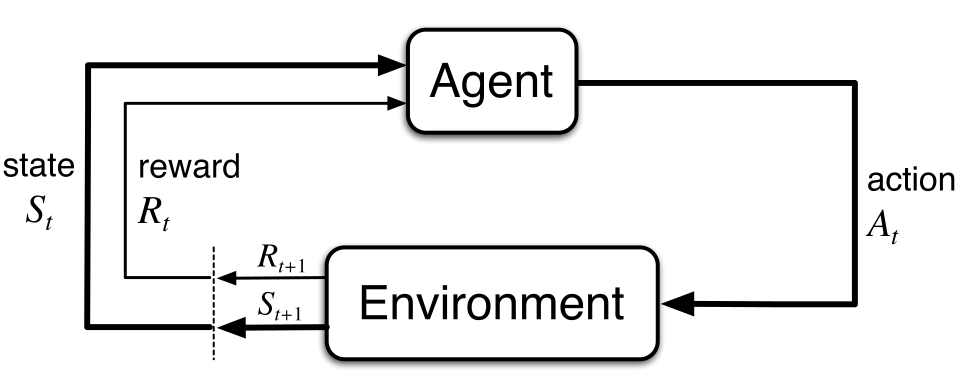
\includegraphics[scale=0.3]{./images/mdp.png}
	\caption{The agent-environment interaction in a Markov decision process.}
	\label{fig:mdp_ill}
\end{figure}

Components of RL:
\begin{itemize}
	\item An agent
	\item A policy
	\item A reward signal: what is good in an immediate sense.
	\item A value function: what is good in the long run.
	\item A model of the environment: This allows inferences to be made about how the environment will behave.
\end{itemize}
%\begin{itemize}
%	\item Agent
%	\item Action
%	\item Environment
%	\item State
%	\item The knowledge of the state is fully observable or partially observable.
%	\item Reward
%	\item Policy
%	\item Episodic task: from an initial state to a terminal state.
%	\item Continuing task: infinite horizon
%\end{itemize}


An MDP is fully characterized by a $\langle S A,P,R,\gamma \rangle$ tuple, where $S$ is a set of states, $P$ is a transition probability matrix, $R$ is a reward function, and $\gamma\in[0,1]$  is a discount factor.

\begin{definition}[Markov Property]
	A state $S_t$ is \textbf{Markov} if and only if 
	$$P[S_{t+1}|S_t, A_t] = P[S_{t+1}|S_t, A_t, S_{t-1},A_{t-1},...]$$
\end{definition}
\begin{itemize}
	\item Actions: a mechanism to influence the environment
	\item State: specific configurations of the environment
\end{itemize}

\begin{definition}[Transition Function]
	$$p(s',r|s,a) = P(S_t=s',R_t=r|S_{t-1}=s,A_{t-1}=a)$$
\end{definition}
\begin{itemize}
	\item The way the environment changes as a response to actions is referred to as the state-transition probabilities, or more simply, the transition function, and is denoted by $T(s,a,s')$.
	\item $\sum_{r\in \mathcal{R}}\sum_{s'\in \mathcal{S}}p(s',r|s,a) = 1, \quad \forall s \in \mathcal{S}, \forall a\in \mathcal{A}(s)$
	\item $p(s'|s,a)=P(S_t=s'|S_{t-1}=s,A_{t-1}=a)=\sum_{r\in \mathcal{R}}p(s',r|s,a)$
\end{itemize}

\begin{definition}[Reward Hypothesis]
	All goals can be described by the maximization of expected cumulative reward.
\end{definition}
\begin{itemize}
	\item That all of what we mean by goals and purposes can be well thought of as athe maximization of the expected value of the cumulative sum of a received scalar signal (called reward).
\end{itemize}

\begin{definition}[Reward Function]
	\begin{align*}
		r(s,a)&= \mathbb{E}[R_t|S_{t-1}=s,A_{t-1}=a]\\
		&= \sum_{r\in \mathcal{R}}r\sum_{s'\in \mathcal{S}}p(s',r|s,a)
	\end{align*}
\end{definition}
\begin{itemize}
	\item $R_t\in \mathcal{R} \subset \mathbb{R}.$ 
		\begin{itemize}
			\item Note that negative reward is still reward.
		\end{itemize}
	\item The expected reward function is defined as a function that takes in a state-action pair.
	\item It is the expectation of reward at time step $t$, given the state-action pair in the previous time step.
	\item The reward function can also be defined as a function that takes a full transition tuple $s,a,s'$.
		\begin{align*}
			r(s,a,s')&= \mathbb{E}[R_t|S_{t-1}=s,A_{t-1}=a,S_{t}=s]\\
			&= \sum_{r\in \mathcal{R}}\frac{p(s',r|s,a)}{p(s'|s,a)}
		\end{align*}
\end{itemize}




\begin{definition}[Discount Factor, $\gamma$]
	$$G_t = R_{t+1}+\gamma R_{t+2}+\gamma^2 R_{t+3}+\cdots+\gamma^{T-1} R_{T} $$
\end{definition}

\begin{itemize}
	\item \textbf{The sum of all rewards obtained during the course of an episode} is referred to as the \textit{return}, $G_t$.
	\item Episodic tasks: $G_t = R_{t+1} + R_{t+2} + \cdots + R_{T}.$
		\begin{itemize}
			\item $G_t = R_{t+1}+\gamma G_{t+1}$
		\end{itemize}
	\item Continuing tasks: $G_t = R_{t+1} + \gamma R_{t+2} +  \gamma^2 R_{t+3} \cdots =\sum_{k=0}^{\infty} \gamma^{k} R_{t+k+1}.$
		\begin{itemize}
			\item $\gamma=0$: myopic evaluation
			\item $\gamma=1$: far-sighted evaluation
			\item Uncertainty about the future that may not be fully observed
			\item Mathematically convenient to discount rewards. 
			\item Avoid infinite returns in cyclic Markov processes.
		\end{itemize}
\end{itemize}

\paragraph{A Simple Example:}
\begin{itemize}
	\item Environment:
		\begin{itemize}
			\item The grid world has 3 states: $S1$, $S2$, and $S3$.
			\item The agent can take actions $A=\{left,right\}$.
			\item The rewards are as follows:
				\begin{itemize}
					\item $R_{left}=−1$: penalty for moving left
					\item $R_{right}=+1$: reward for moving right
				\end{itemize}
			\item The discount factor $\gamma$: 0.9.
		\end{itemize}
	\item Episode:
		\begin{enumerate}
			\item The agent starts in $S1$.
			\item If the agent moves left, it incurs a penalty ($R_{left}=−1$), and the episode ends.
			\item If the agent moves right, it receives a reward ($R_{right}=+1$), transitions to $S2$, and the episode continues.
			\item In $S2$, the agent faces the same choices.
			\item The episode ends when the agent either moves left or reaches $S3$.
		\end{enumerate}
	\item Return Calculation:
		\begin{itemize}
			\item Let's calculate the return for a sample trajectory: $\{S1,right,S2,right,S3\}$.
			\item $G=R_{right}+\gamma R_{right}+\gamma^2R_{right}=2.71$ 
			\item So, the return for this trajectory is 2.71.
		\end{itemize}
\end{itemize}

\section{Policies and Value Functions}
\begin{itemize}
	\item Policies are universal plans, which provides all possible plans for all states. 
		\begin{itemize}
			\item Plans are not enough to fully describe an environment in stochastic environments.
				\begin{itemize}
					\item What if an agent intends to move right, but ends up going left. Which action does the agent take?
				\end{itemize}
			\item Policies are the per-state action descriptions.
			\item Policy can be stochastic or deterministic.
			\item A policy is a function that prescribes actions to take for a given non-terminal state.
		\end{itemize}
\end{itemize}

Formally, a policy is a mapping from states to probabilities of selecting each possible action. It can be defined 
$$\pi(a|s)$$

\subsection{The State-Value Functions}

Almost all reinforcement learning algorithms involve estimating \textit{value functions}, functions of states (or of state-action pairs) that estimate how good it is for the agent to be in a given state (or how good it is to perform a given action in a given state). The notion of ``how good'' here is defined in terms of future rewards that can be expected, or, to be precise, in terms of \textbf{expected return}. Sure, we want high returns, but high in expectation (on average). Of course, the rewards the agent can expect to receive in the future depend on what actions it will take. Accordingly, value functions are defined with respect to particular ways of action, called policies. 

\begin{definition}[The State-Value Function, $V$]
	The state-value function $v(s)$ for policy $\pi$ of an Markov Reward Process is the expected return starting from state $s$
	\begin{align*}
		v_{\pi}(s) &= \mathbb{E}_\pi[G_t|S_t=s]\\
				   &= \mathbb{E}_\pi \Bigg[\sum_{k=0}^\infty \gamma^kR_{t+1+k}\Big|S_t=s\Bigg], \quad \forall s\in \mathcal{S}
				   % &= \mathbb{E}_\pi \Bigg[R_{t+1}+\gamma G_{t+1}\sum_{k=1}^\infty \gamma^kR_{t+1+k}\Big|S_t=s\Bigg], \quad \forall s\in \mathcal{S}\\
	\end{align*}
	$$$$
\end{definition}

\begin{itemize}
	\item The value of a state $s$ is the expectation over policy $\pi$.
	\item Value function is the expected return. 
		\begin{itemize}
			\item Reward: one-step signal that an agent receives.
			\item Return: total discounted rewards, which is the sum of rewards obtained from time $t$ onward.
		\end{itemize}
	\item If we are given a policy and the MDP, we should be able to calculate the expected return starting from every single state. 
\end{itemize}

The state-value function satisfies the \textit{Bellman equation}, which expresses the relationship between the value of a state and the values of its successor states:
\begin{align}
	v_\pi(s) &= \mathbb{E}_\pi[G_t|S_t=s]\\
	& = \mathbb{E}_\pi[R_{t+1} + \gamma G_{t+1}|S_t=s]\\
	% & = \mathbb{E}_\pi[R_{t+1} + \gamma v(s_{t+1})|S_t=s]\\
	& = \sum_{a}\pi(a|s)\sum_{s',r}p(s',r|s,a)[r + \gamma v_\pi(s')],\, \forall s \in \mathcal{S}.
	\label{eq:state_value_bellman}
\end{align}
For better understanding, let's look at the \Cref{fig:state_value_diagram}. Starting from state $s$, the root node at the top, the agent could take any of some set of actions (three actions are shown in the diagram), based on its policy $\pi$. From each of these, the environment could respond with one of several next states, $s'$ (two states are shown in the figure), along with a reward, $r$, depending on its dynamics given by the function $p$. The Bellman equation averages over all the possibilities, weighting each by its probability of occurring. \textbf{It states that the value of the start state must equal (discounted) the value of the expected next state, plus the reward expected along the way}. 
\begin{figure}[h]
	\centering
	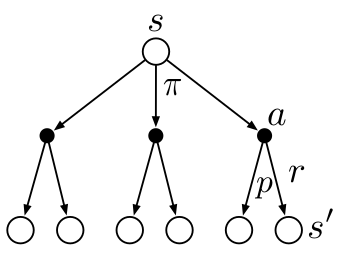
\includegraphics[scale=0.3]{./images/backup_vpi.png}
	\label{fig:state_value_diagram}
\end{figure}
The derivation of \Cref{eq:state_value_bellman} is given in \Cref{appendix:bellman_equation}. The state-value function is essential for understanding the value of different states in a Markov Decision Process (MDP) and is often used in various reinforcement learning algorithms, such as value iteration and policy iteration.

% The Bellman equation for the state-value function can be expressed in matrix form as follows:
% \begin{align}
% 	v_\pi(s) &= \mathbb{E}_\pi[G_t|S_t=s]\\
% 	& = \mathbb{E}_\pi[R_{t+1} + \gamma G_{t+1}|S_t=s]\\
% 	& = \mathbb{E}_\pi[R_{t+1} + \gamma v(s_{t+1})|S_t=s]\\
% 	% & = \sum_{a}\pi(a|s)\sum_{s',r}p(s',r|s,a)[r + \gamma v_\pi(s')],\, \forall s \in \mathcal{S}.
% 	% \label{eq:state_value_bellman}
% \end{align}




\subsection{The Action-Value Function}
\begin{itemize}
	\item Another critical question that we often need to ask is not merely about the value of a state but the value of taking action $a$ at a state $s$.
	\item Which action is better under each policy?
	\item The action-value function, also known as $Q$-function or $Q^\pi(s,a)$, captures precisely this.
		\begin{itemize}
			\item The expected return if the agent follows policy $\pi$ after taking action $a$ in state $s$.
		\end{itemize}
\end{itemize}

\begin{definition}[The Action-Value Function, $Q$]
	The action-value function $q_{\pi}(s,a)$ for policy $\pi$ is the expected return starting from state $s$, tacking action $a$ under policy $\pi$
	$$q_{\pi}(s,a) = \mathbb{E}_\pi[G_t|S_t=s, A_t=a]=\mathbb{E}_\pi\Bigg[\sum_{k=0}^{\infty}\gamma^k R_{t+k+1}\Bigg| S_t=s, A_t=a\Bigg]$$
\end{definition}

\begin{itemize}
	\item The Bellman equation for the action-value function is given by
	\begin{align*}
		q_{\pi}(s,a) &= \mathbb{E}_\pi[G_t|S_t=s, A_t=a]\\
		& = \mathbb{E}_\pi[R_{t+1} + \gamma G_{t+1}|S_t=s, A_t=a]\\
		& = \sum_{s',r}p(s',r|s,a)[r + \gamma v_\pi(s')]
	\end{align*}
	\item Notice that we do not weight over actions because we are interested only in a specific action.
	\item The action-value function is crucial for understanding the value of different state-action pairs in a Markov Decision Process (MDP) and is used in various reinforcement learning algorithms, such as Q-learning and deep Q-networks (DQN).
	\item The derivation is given in \Cref{appendix:bellman_equation}
\end{itemize}

The state-value function can be also expressed by using the action-value function as follows:
\begin{align*}
	v_\pi(s) &= \mathbb{E}_{\pi}[G_t|S_t = s]\\ 
	&= \sum_{g_t} g_t\cdot P[G_t|S_t=s]\\
	&= \sum_{g_t} g_t\cdot P[G_t,S_t=s]/P[S_t=s]\\
	&= \sum_{g_t} g_t\cdot \sum_a P[G_t,S_t=s, A_t=a]/P[S_t=s]\\
	&= \sum_{g_t} g_t\cdot \sum_a \Big[P[G_t|S_t=s, A_t=a]P[S_t=s, A_t=a]\Big]/P[S_t=s]\\
	%&= \sum_{g_t} g_t \sum_a P(G_t|S_t=s, A_t=a) P(A_t=a|S_t=s)\\
	&= \sum_{g_t} g_t \sum_a P[G_t, A_t=a|S_t=s] P[A_t=a|S_t=s]\\
	&= \sum_{a} \sum_{g_t} g_t P[G_t|S_t=s, A_t=a] P[A_t=a|S_t=s]\\
	&= \sum_{a} q_\pi(s,a) \pi(a|s)
\end{align*}
Note that the expectation is parameerized $\pi$ as written in $\mathbb{E}_{\pi}$. We can also simply prove it by the \textit{Law of Total Expectation} \footnote{
$\mathbb{E}[\mathbb{E}[X|Y]] = \sum_{y}\Big[\sum_{x}x\cdot\ p(X=x|Y)\Big] p(Y=y) = \mathbb{E}[X]$},
\begin{align*}
	v_\pi(s) &= \mathbb{E}_{\pi}[G_t|S_t = s]\\ 
	&= \mathbb{E}[\mathbb{E}_{\pi}[G_t|S_t=s, A_t=a]]\\
	&= \sum_{a} \mathbb{E}_{\pi}[G_t|S_t=s, A_t=a] P(A_t = a|S_t = s)\\
	&= \sum_{a} q_\pi(s,a) \pi(a|s)
\end{align*}
An intuitive explantation of this derivation is that the expectation depends on an action $a\sim \pi(a|s)$. We want to estimate the expected total return by the sampled action (this is because the total return is the function of $a$, implicitly). Then, we need to introduce an action variable $a$ and its probability in the expression as the second line of the equation. 

\subsection{The Action-Advantage Function}

\begin{definition}[The Action-Advantage Function, $A$]
	$$a_{\pi}(s,a) = q_\pi(s,a)-v_\pi(s)$$
\end{definition}

The advantage function describes how much better it is to take action $a$ instead of following policy $\pi$. In other words, the advantage of choosing action $a$ over the default action, set by the policy.

\section{Optimality}

Solving a reinforcement learning task means, roughly, finding a policy that achieves a lot of reward over the long run. For finite MDPs, we can precisely define an optimal policy in the following way. Value functions define a partial ordering over policies. A policy $\pi$ is defined to be better than or equal to a policy $\pi'$ if its expected return is greater than or equal to that of $\pi'$ for all states. In other words, $\pi\geq \pi'$ if and only if $v_\pi(s)\geq v_{\pi'}(s)$ for all $s\in \mathcal{S}$. There is always at least one policy that is better than or equal to all other policies. This is an \textit{optimal policy}. The optimal state-value function, denoted $v_*$ can be defined as 


\begin{definition}[Optimal State-Value Function]
	The optimal state-value function $v_{*}(s)$ is the maximum value over all policies
	$$v_{*}(s) = \max_{\pi} v_{\pi}(s),\quad \forall s\in \mathcal{S}.$$
\end{definition}

\begin{itemize}
	\item The optimal state-value function can be obtained as follows:
%		\begin{align*}
%			v_{*}(s)&= \max_{a\in\mathcal{A}(s)} q_*(s,a)\\
%			&= \max_a \sum_{s',r}p(s',r|s,a)[r + \gamma v_*(s')]
%		\end{align*}

		\begin{align*}
			v_*(s) &= \max_{a\in \mathcal{A}(s)}q_{\pi_*}(s,a)\\
			&= \max_a \mathbb{E}_{\pi_*}[G_t| S_t=s, A_t=a]\\
			&= \max_a \mathbb{E}_{\pi_*}[R_{t+1}+\gamma G_{t+1}| S_t=s, A_t=a]\\
			&= \max_a \mathbb{E}_{\pi_*}[R_{t+1}+\gamma v_*(S_{t+1})| S_t=s, A_t=a]\\
			&= \max_a \sum_{r,s'}p(s',r|s,a)\Big[r + \gamma  v_*(s')\Big] 
	\end{align*}

\end{itemize}

\begin{definition}[Optimal Action-Value Function]
	The optimal action-value function $q_{*}(s, a)$ is the maximum value over all policies
	$$q_{*}(s,a) = \max_{\pi} q_{\pi}(s,a), \quad \forall s\in \mathcal{S} \textrm{ and } a\in \mathcal{A}.$$
\end{definition}
\begin{itemize}
	\item The optimal action-value function can be obtained as follows:
		\begin{align*}
		q_{*}(s,a) &= \mathbb{E}[R_{t+1}+\gamma v_*(S_{t+1})|S_t=s, A_t=a]\\
		&= \sum_{s',r}p(s',r|s,a)[r + \gamma \max_a q_*(s',a')]
		\end{align*}
		\begin{figure}[h]
			\centering
			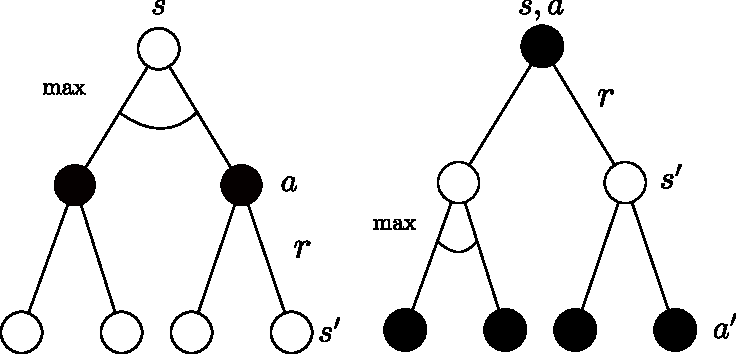
\includegraphics[scale=0.5]{./images/optimal_action.pdf}
		\end{figure}
	\item The optimal value function specifies the best possible performance in the MDP.
	\item The MDP is solved when we know the optimal value function
\end{itemize}

\begin{theorem}[Optimal Policy Theorem]
	$$\pi\geq \pi' \quad\textrm{if}\quad v_\pi(s) \geq v_{\pi'}(s), \forall s$$
	For any Markov Decision Process:
	\begin{itemize}
		\item There exists an optimal policy $\pi_*$ that is better than or equal to all other policies, $\pi_*\geq \pi, \forall \pi$
		\item All optimal policies achieve the optimal value function, $v_{\pi_*}(s) = v_*(s)$
		\item All optimal policies achieve the optimal action-value function, $q_{\pi_*}(s,a) = q_{*}(s,a)$
	\end{itemize}
\end{theorem}

An optimal policy can be found by maximizing over $q_*(s,a)$, 
\begin{align*}
	\pi_*(a|s) = 
	\begin{cases} 
		&1 \quad \textrm{if } a = \argmax_{a\in \mathcal{A}}q_*(s,a)\\
		&0 \quad \textrm{otherwise}
	\end{cases}
\end{align*}
\begin{itemize}
	\item There is always a deterministic optimal policy for any MDP
	\item If we know $q_*(s,a)$, we immediately have the optimal policy 
		\begin{itemize}
			\item Q-learning: learns Q values first
			\item Policy gradient: learns optimal policy without learning Q values
		\end{itemize}
\end{itemize}


\chapter{Dynamic Programming}
The term dynamic programming (DP) refers to a collection of algorithms that can be used to compute optimal policies given a perfect model of the environment as a Markov decision process (MDP). Classical DP algorithms are of limited utility in reinforcement learning both because of their assumption of a perfect model and because of their great computational expense, but they are still important theoretically. The key idea of DP, and of reinforcement learning generally, is the use of value functions to organize and structure the search for good policies.


Let $\pi$ and $\pi'$ be any pair of deterministic policies such that, for all $s\in \mathcal{S}$, 
\begin{align*}
	q_\pi(s, \pi'(s))\geq v_\pi(s).	
\end{align*}
Then, the policy $\pi'$ must be as good as, or better than $\pi$. Equivalently, it must obtain the following inequality for all states $s\in \mathcal{S}$:
\begin{align*}
	v_\pi'(s)\geq v_\pi(s).	
\end{align*}

\begin{theorem}[Policy Improvement Theorem]
	If $q_\pi(s, \pi'(s))\geq v_\pi(s)$, then 
	$$v_\pi'(s)\geq v_\pi(s)$$
	\label{thrm:policy_improvement}
\end{theorem}
%Proof.

%\begin{align*}
%	v_\pi(s)&\leq q_\pi(s, \pi'(s))	\\
%	&= \mathbb{E}[R_{t}+\gamma v_\pi(S_{t+1})|S_t=s, A_t=\pi'(s)]\\
%	&= \mathbb{E}_{\pi'}[R_{t}+\gamma v_\pi(S_{t+1})|S_t=s]\\
%	&\leq \mathbb{E}_{\pi'}[R_{t}+\gamma q_\pi(S_{t+1}, \pi'(S_{t+1}))|S_t=s]\\
%	&= \mathbb{E}_{\pi'}[R_{t}+\gamma \mathbb{E}_{\pi'}[R_{t+2}+\gamma v_\pi(S_{t+2})|S_{t+1}, A_{t+1}=\pi'(S_{t+1})]\,|\,S_t=s]\\
%	&= \mathbb{E}_{\pi'}[R_{t}+\gamma R_{t+2}+\gamma^2 v_\pi(S_{t+2})|\,S_t=s]\\
%	&\leq \mathbb{E}_{\pi'}[R_{t}+\gamma R_{t+2}+\gamma^2 R_{t+3}+\gamma^3 v_\pi(S_{t+3})|\,S_t=s]\\
%	&\vdots\\
%	&\leq \mathbb{E}_{\pi'}[R_{t}+\gamma R_{t+2}+\gamma^2 R_{t+3}+\gamma^3 R_{t+4}+\ldots|\,S_t=s]\\
%	&= \mathbb{E}_{\pi'}[G_t|\,S_t=s]\\
%	&= v_{\pi'}(s).
%	%\label{eq:policy_improvement_theorem}
%\end{align*}


\section{Policy Evaluation}
\begin{itemize}
	\item Prediction problem: refers to the problem of \textbf{evaluating policies} (sipmly, rating policies), of estimating value functions given a policy (learning to predict returns).
	\item Control problem: problem of \textbf{finding optimal policies}. Usually solved by the pattern of generalized policy iteration (GPI), where the competing processes of policy evaluation and policy improvement progressively move policies towards optimality.
	\item Policy evaluation: refers to algorithms that solve the prediction problem.
		\begin{itemize}
			\item Iterative policy evaluation:
				$$v_{k+1}(s)=\sum_{a}\pi(a|s)\sum_{s'}p(s'|s,a)[r + \gamma v_k(s')].$$ 
				\begin{enumerate}
					\item Init $v_0(s)$ for all $s$ arbitrarily and to 0 if $s$ is terminal. 
					\item Bootstrapping: $v_1(s)\to v_2(s)\to\cdots\to v_N(s)$
				\end{enumerate}
		\end{itemize}
\end{itemize}

A single round of updates, $k$ , involves updating all the state values. The algorithm stops until 
the changes in state values are sufficiently small in successive iterations.

% \section{Policy Iteration}

\section{Policy Improvement}
Our reason for computing the value function for a policy is to help find better policies. The goal of policy improvement is to modify the policy to make it better with respect to the value function. This is done by selecting actions that are known to be better, according to the current value estimates.

\begin{itemize}
	\item The key is the action-value function, $q_\pi(s,a)$. To improve a policy, we use a state-value function and an MDP to get a one-step look-ahead and determine which of the actions lead to the highest value. We can selects the action that \textit{maximizes the action-value function in a greedy way}: 
		\begin{align*}
			\pi'(s) &= \argmax_a q_\pi(s,a)\\
			&= \argmax_a \sum_{s'}p(s'|s,a)[r + \gamma v_\pi(s')].
		\end{align*}
	\item The greedy policy takes the action that looks best in the short term according to $v_\pi$.
	\item If the policy is not going to be updated, then the policy is the optimal policy.
\end{itemize}

The process of policy evaluation and improvement is often repeated iteratively until the policy converges to an optimal policy that maximizes the expected return in the given environment. This iterative process is the basis for algorithms like \textit{policy iteration} and \textit{value iteration} in reinforcement learning.


\section{Value Iteration}
One drawback to policy iteration is that each of its iterations involves policy evaluation, which may itself be a protracted iterative computation requiring multiple sweeps through the state set.

In fact, the policy evaluation step of policy iteration can be truncated in several ways without losing the convergence guarantees of policy iteration.

\begin{align}
	v_{k+1}(s)=\max_a \sum_{s'}p(s'|s,a)[r + \gamma v_k(s')], \, \forall s\in \mathcal{S}.
	\label{eq:value_iteration}
\end{align}
For arbitrary $v_0$, the sequence $v_k$ can be shown to converge to $v_*$ under the same conditions that guarantee the existence of $v_*$.


\chapter{Monte Carlo Methods}
% Our goal is to estimate value functions and find optimal policies. Monte-Carlo methods require only \textit{experience}--sample sequences of states, actions, and rewards from actual or simulated interaction with an environment. 
Monte Carlo methods are a class of computational algorithms that rely on random sampling to obtain numerical results. In the context of reinforcement learning (RL), Monte Carlo methods are often used to estimate the value of states or state-action pairs in a Markov Decision Process (MDP).


\section{Monte Carlo Prediction (Evaluation)}
% Recall that the value of a state is the expected return starting from that state. An obvious way to estimate it from experience, then, is simply to average the returns observed after visits to that state. As more returns are observed, the average should converge to the expected value. This idea is the core of Monte Carlo methods. 
The goal is to estimate the value of a policy, that is, to learn how much total reward to expect from a policy. 

The most straightforward approach that comes to mind is one I already men- tioned: it’s to run several episodes with this policy collecting hundreds of trajectories, and then calculate averages for every state, just as we did in the bandit environments. This method of estimating value functions is called Monte Carlo prediction (MC).


\subsection{First Visit vs. Every Visit}
Suppose we wish to estimate $v_\pi(s)$, the value of a state $s$ under policy $\pi$, given a set of episodes obtained by following $\pi$ and passing through $s$. Each occurrence of state $s$ in an episode is called a visit to $s$. 

\paragraph{The first-visit MC} method estimates $v_\pi(s)$ as the average of the returns following first visits to $s$, whereas \textit{the every-visit MC} method averages the returns following all visits to $s$.

\begin{itemize}
	\item First visit MC treats each trajectory as an i.i.d., sample of $v(s)$.
	\item For instance, we have two example episodes, 
		\begin{itemize}
			\item $A, 3\to A, 2\to B, -4\to A, 4\to B, -3$.
			\item $B, -2\to A, 3\to B, -3$.
		\end{itemize} 
	\item Each number next to the states are reward. Let's say discount factor is 1 and we want to compute $V(A)$, then the first visit MC computes a return by summing all the rewards ($G\leftarrow \gamma G + R_{t+1}$) coming after the first visit to the state $A$. Therefore, we can't have more than one summation term for each episode for a state. In sum,
	\begin{itemize}
		\item For the first episode: $3+2-4+4-3=2$.
		\item For the second episode: $3-3=0$.
		\item Thus, $V(A) = (2+0)/2=1$.
		\item It must be noted that if an episode doesn't have an occurrence of `$A$', it won't be considered in the average. Hence if a 3rd episode is given like $B,3\to B,3\to terminate$ existed, still $V(A)=1$.
	\end{itemize}
\end{itemize}

\begin{figure}[h]
	\centering
	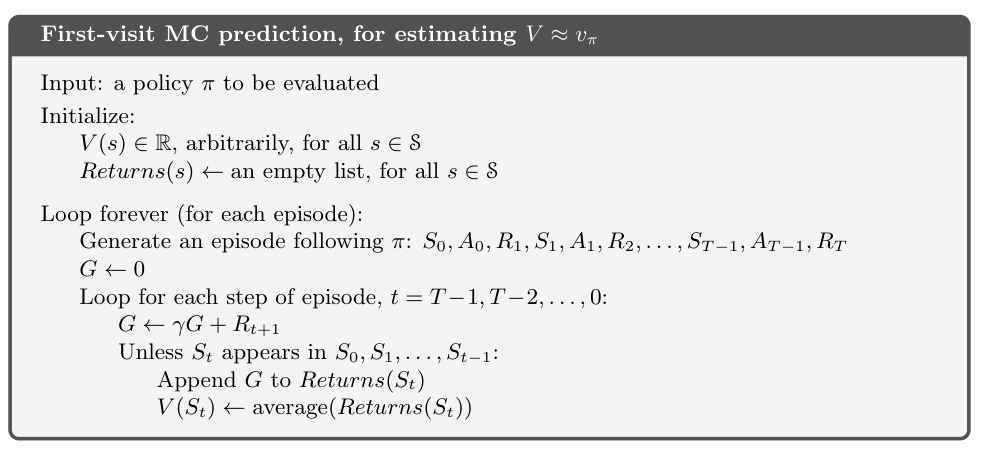
\includegraphics[scale=0.5]{./images/first_visit_mc.png}
	\caption{First-visit MC prediction algorithm.}
	\label{fig:first_visit_mc}
\end{figure}

\paragraph{Every visit MC} method averages the returns following \textbf{all visits} to $s$.
\begin{itemize}
	\item Here, we would be creating a new summation term adding all rewards coming after every occurrence of `$A$'(including that of $A$ as well).
		\begin{itemize}
			\item From 1st episode: $(3+2-4+4-3)+(2-4+4-3)+(4-3)=2-1+1$
			\item From 2nd episode: $(3-3)=0$
			\item As we got 4 summation terms, we will be averaging using $N=4$ \ie
			\item $V(A)=(2-1+1+0)/4=0.5$
		\end{itemize}
\end{itemize}



\section{Monte Carlo Control}
$$\pi_0\xrightarrow{\,E\,} q_{\pi_0} \xrightarrow{\,I\,} \pi_0\xrightarrow{\,E\,} q_{\pi_0}\xrightarrow{\,I\,}\cdots \xrightarrow{\,I\,} \pi_*\xrightarrow{\,E\,} q_{\pi_*},$$
\begin{itemize}
	\item $\pi_0$: arbitrary policy.
	\item Policy improvement is done by making the policy greedy with respect to the current value function (action-value function). 
	\item For any action-value function $q$, the corresponding greedy policy is the one that, for each $s\in \mathcal{S}$, deterministically chooses an action with maximal action-value:
		$$\pi(S) = \argmax_a q(s,a).$$
	\item Policy improvement then can be done by constructing each $\pi_{k+1}$ as the greedy policy with respect to $q_{\pi_k}.$
	\item By \Cref{thrm:policy_improvement}, each $\pi_{k+1}$ is uniformly better than $\pi_k$ or just as good as $\pi_k$.
\end{itemize}


\section{On-Policy vs. Off-Policy}
%Monte Carlo prediction (or evaluation) is used to evaluate the value of a given policy, while Monte Carlo control is for finding the optimal policy when such a policy is not given. There are two categories of MC control:
\paragraph{On-policy} learns about the optimal policy by executing the policy and evaluating and improving it.  
\begin{itemize}
	\item Learning to be great by itself.
	\item The agent learns from the experiences it gathers while following its current policy.
	\item The policy is typically denoted by $\pi$.
	\item The learning process is directly tied to the policy being used for action selection.
	\item Examples of on-policy algorithms include REINFORCE (Monte Carlo Policy Gradient) and Proximal Policy Optimization (PPO).
	\end{itemize}

\paragraph{Off-policy} learns about the optimal policy by using data generated by another policy. 
\begin{itemize}
	\item Learning from others.
	\item The agent can learn from historical data, which may have been generated by an older policy.
	\item The policy used for learning is not necessarily the one used for action selection.
	\item The data collected can be more efficiently reused for learning new policies.
	\item Examples of off-policy algorithms include Q-learning, Deep Q Networks (DQN), and Actor-Critic methods.
\end{itemize}


\paragraph{Exploration-Exploitation Trade-off}
\begin{itemize}
	\item On-policy algorithms often struggle with exploration because they are committed to following their current policy, which may not explore the state space efficiently.
	\item Off-policy algorithms can be more sample-efficient in exploration as they can learn from a mixture of data from different policies.
\end{itemize}

\paragraph{Data Efficiency}
\begin{itemize}
	\item Off-policy algorithms can potentially be more data-efficient since they can reuse past experiences collected by any policy.
	\item On-policy algorithms typically require more samples to update the policy effectively.
\end{itemize}
    
\paragraph{Stability and Convergence}
\begin{itemize}
	\item On-policy algorithms can be more stable because they are directly optimizing the policy they are following.
	\item Off-policy algorithms might face challenges related to the stability of learning, especially when dealing with function approximation, as is often the case with deep learning.
\end{itemize}
    
Both on-policy and off-policy algorithms have their strengths and weaknesses, and the choice between them depends on the specific requirements and characteristics of the problem at hand.

\section{Exploration-Exploitation Trade-off}
The more episodes are collected, the better, but there is a problem. If the algorithm for policy improvement always updates the policy greedily, meaning it takes only actions leading to immediate reward, actions and states not on the greedy path will not be sampled sufficiently, and potentially better rewards would stay hidden from the learning process.

Essentially, we are forced to make a choice between making the best decision given the current information or start exploring and finding more information. This is also known as the Exploration vs. Exploitation Dilemma.

We are looking for something like a middle ground between those. Full-on exploration would mean that we would need a lot of time to collect the needed information, and full-on exploitation would make the agent stuck into a local reward maximum. There are two approaches to ensure all actions are sampled sufficiently called on-policy and off-policy methods.



\subsection{On Policy}
On-policy methods solve the exploration vs exploitation dilemma by including randomness in the form of a policy that is soft, meaning that non-greedy actions are selected with some probability. These policies are called $\epsilon$-greedy policies as they select random actions with an $\epsilon$ probability and follow the optimal action with $1-\epsilon$ probability

Since the probability of selecting from the action space randomly is $\epsilon$, the probability of selecting any particular non-optimal (non-greedy) action is $\epsilon/|\mathcal{A}(s)|$. The probability of following the optimal action will always be slightly higher, however, because we have a $1 - \epsilon$ probability of selecting it outright and $\epsilon/ |\mathcal{A}(s)|$ probability of selecting it from sampling the action space \footnote{Since the greedy (or optimal) action can be selected by either 1-$\epsilon$ or $\epsilon/ |\mathcal{A}(s)|$, $a_1=\epsilon/\mathcal{A}(s),a_2=\epsilon/\mathcal{A}(s),\cdots,a_{best}=1-\epsilon+\epsilon/\mathcal{A}(s),a_n = \epsilon/\mathcal{A}(s)$}
$$P(a_t^{*}) = 1 - \epsilon+\epsilon/ |\mathcal{A}(s)|.$$
It is also worth noting that because the optimal action will be sampled more often than the others making on-policy algorithms will generally converge faster but they also have the risk of trapping the agent into a local optimum of the function.

%On-Policy learning algorithms are the algorithms that evaluate and improve the same policy which is being used to select actions. That means we will try to evaluate and improve the same policy that the agent is already using for action selection. In short , [Target Policy == Behavior Policy]. Some examples of On-Policy algorithms are Policy Iteration, Value Iteration, Monte Carlo for On-Policy, Sarsa, etc.

\subsection{Off Policy}

All learning control methods face a dilemma: They seek to learn action values conditional on subsequent \textit{optimal} behavior, but they need to behave non-optimally in order to explore all actions (to find the optimal actions). How can they learn about the optimal policy while behaving according to an exploratory policy? The on-policy approach in the preceding section is actually a compromise. It learns action values not for the optimal policy, but for a near-optimal policy that still explores. A more straightforward approach is to \textbf{leverage two policies}, one that is learned about and that becomes the optimal policy, and one that is more exploratory and is used to generate behavior. The policy being learned about is called the \textit{target policy}, and the policy used to generate behavior is called the \textit{behavior policy}. In this case we say that learning is from data ``off'' the target policy, and the overall process is termed \textit{off-policy learning}.

Suppose we wish to estimate $v_\pi$ or $q_\pi$, but all we have are episodes following another policy $b$, where $b\neq \pi$. In this case, $\pi$ is the target policy, $b$ is the behavior policy, and both policies are considered fixed and given. 

In order to use episodes from $b$ to estimate values for $\pi$, we require that every action taken under $\pi$ is also taken, at least occasionally, under $b$. That is, we require that $\pi(a|s) > 0$ implies $b(a|s) > 0$. This is called the assumption of \textit{coverage}. It follows from coverage that $b$ must be stochastic in states where it is not identical to $\pi$. The target policy $\pi$, on the other hand, may be deterministic, and, in fact, this is a case of particular interest in control applications. In control, the target policy is typically the deterministic greedy policy with respect to the current estimate of the action-value function. This policy becomes a deterministic optimal policy while the behavior policy remains stochastic and more exploratory, for example, an $\epsilon$-greedy policy. %In this section, however, we consider the prediction problem, in which ⇡ is unchanging and given.

Almost all off-policy methods utilize \textit{importance sampling}, a general technique for \textbf{estimating expected values under one distribution given samples from another}. We apply importance sampling to off-policy learning by weighting returns according to the relative probability of their trajectories occurring under the target and behavior policies, called the \textit{importance-sampling ratio}. Given a starting state $S_t$, the probability of the subsequent state-action trajectory, $A_t, S_{t+1}, A_{t+1},\cdots,S_T$, occurring under any policy $\pi$ is 
\begin{align*}
	P(A_t, S_{t+1}, A_{t+1},\cdots,S_T)&= \pi(A_t|S_t)p(S_{t+1}|S_t,A_t)\pi(A_{t+1}|S_{t+1})\cdots(S_T|S_{T-1},A_{T-1})\\ 
	&= \prod_{k=t}^{T-1}\pi(A_k|S_k)p(S_{k+1}|S_k,A_k),
\end{align*}
where $p$ here is the state-transition probability function. Thus, the relative probability $\rho$ of the trajectory under the target ($\pi$) and behavior policies ($b$) is 
\begin{align*}
	\rho_{t:T-1} &=  \frac{\prod_{k=t}^{T-1}\pi(A_k|S_k)p(S_{k+1}|S_k,A_k)}{ \prod_{k=t}^{T-1}b(A_k|S_k)p(S_{k+1}|S_k,A_k)}\\
	&= \prod_{k=t}^{T-1}\frac{\pi(A_k|S_k)}{b(A_k|S_k)}.
\end{align*}
The importance sampling ratio ends up depending only on the two polices and the sequence, not on the MDP's state-transition probability.

Recall that we wish to estimate the expected returns under the target policy, but all we have are returns $G_t$ from the behavior policy, which results in 
\begin{align*}
	\mathbb{E}[G_t|S_t=s] = v_b(s).
\end{align*}

So, the ratio $\rho_{t:T-1}$ transforms the returns
\begin{align*}
	\mathbb{E}[\rho_{t:T-1} G_t|S_t=s] = v_\pi(s).
\end{align*}

\section{Temporal-Difference Learninig}
One of the central ideas of reinforcement learning is temporal-difference (TD) learning. TD learning is a combination of Monte Carlo ideas and dynamic programming (DP) ideas. Like Monte Carlo methods, TD methods can learn directly from raw experience without a model of the environment's dynamics. Like DP, TD methods update estimates based in part on other learned estimates, without waiting for a final outcome (they bootstrap). 

One of the main drawbacks of MC methods is the fact that the agent has to wait until the end of an episode when it can obtain the actual $G_t$. Then, it uses that return as a target for $V(S_t)$.


The core of TD learning is the Temporal Difference (TD) error, denoted as $\delta_t$, which represents the difference between the estimated value of a state at time $t$ and the estimated value at time $t+1$. It is calculated as the difference between the reward at time $t+1$ and the discounted estimate of the value function at time $t$.

Constant-$\alpha$ MC:
$$V(S_t) \leftarrow V(S_t)+ \alpha \Big[G_t-V(S_t)\Big] $$

One-step TD (or TD(0)):
$$V(S_t) \leftarrow V(S_t)+ \alpha \Big[\underbrace{R_{t+1}+\gamma V(S_{t+1})-V(S_t)}_{\text{TD error, $\delta$}}\Big] $$

To clarify the difference, let's consider a simple example of a grid-world navigation task. 

\paragraph{MC Method} The agent explores the grid-world and reaches a target goal ($S_9$). The episode ends, and the agent receives a reward of +1. At the end of the episode, the agent updates the value of each visited state based on the observed return. If the trajectory is $S_1\to S_2 \to \cdots\to S_9$, then the value update for each visited state would be based on the return of +1.

\paragraph{TD Learning} The agent starts at $S_1$, moves to $S_2$, and receives a reward of $-0.1$ for the movement. The agent updates the value of $S_1$ based on the observed TD error, which is the immediate reward plus the discounted estimate of the next state. If the agent moves right from $S_1$ to $S_2$, the update for $S_1$ would be based on $R_{move}+\gamma V(S_2)$.

\begin{itemize}
	\item Monte Carlo:
		\begin{itemize}
			\item Pros: Unbiased estimate of value functions.
			\item Cons: Requires complete episodes, might be computationally expensive.
		\end{itemize}
	\item Temporal Difference:
		\begin{itemize}
			\item Pros: Updates at each time step, more sample-efficient.
			\item Cons: Potential bias due to bootstrapping.
		\end{itemize}
\end{itemize}
In summary, in the grid-world example, Monte Carlo methods would update values based on complete episodes, whereas TD learning would update values at each time step. The choice depends on the nature of the task, the availability of information, and the computational resources.

\begin{lstlisting}[language=Python]
import numpy as np
import random

def random_walk_environment(state):
    """
    Given the current state (1..5), this environment transitions left or right 
    with equal probability and returns the next state, as well as the reward.
    
    Args:
        state (int): Current non-terminal state, 1 <= state <= 5.
    
    Returns:
        next_state (int): Next state in {0,1,2,3,4,5,6}.
        reward (float): Reward for the transition.
    """
    # Action: move left (prob=0.5) or right (prob=0.5)
    action = random.choice([-1, +1])
    next_state = state + action

    # If next_state == 6, reward = +1; if next_state == 0, reward = 0
    # For states 1..5, reward = 0
    if next_state == 6:
        reward = 1.0
    else:
        reward = 0.0
    
    return next_state, reward


def td_zero_random_walk(num_episodes=1000, alpha=0.1, gamma=1.0):
    """
    Perform TD(0) to evaluate the value function V(s) for the random walk example.
    
    Args:
        num_episodes (int): Number of episodes to run.
        alpha (float): Step-size / learning rate.
        gamma (float): Discount factor (set to 1.0 in the classic random walk).
    
    Returns:
        V (np.array): Learned value function estimates V(s) for states s in [0..6].
                      Terminal states 0 and 6 stay at V=0 by definition.
    """
    # We track V(s) for states 0..6, but 0 and 6 are terminal.
    # Initialize with zeros (you could initialize them differently).
    V = np.zeros(7)

    for episode in range(num_episodes):
        # Start each episode in the middle state (often chosen as 3 in the random walk)
        state = 3

        # Continue until we reach a terminal state
        while state not in [0, 6]:
            next_state, reward = random_walk_environment(state)

            # TD(0) update:
            # V[s] <- V[s] + alpha * [R + gamma * V[s'] - V[s]]
            V[state] = V[state] + alpha * (reward + gamma * V[next_state] - V[state])

            state = next_state

    return V

if __name__ == "__main__":
    # Set random seed for reproducibility (optional)
    random.seed(42)
    np.random.seed(42)

    # Run TD(0) for 1000 episodes
    num_episodes = 1000
    alpha = 0.1
    V_estimates = td_zero_random_walk(num_episodes, alpha)

    print(f"Value Function Estimates after {num_episodes} episodes:")
    for s in range(7):
        print(f"V({s}) = {V_estimates[s]:.3f}")
\end{lstlisting}


\subsection{Q-learning: Off-policy TD Control}

$$Q(S_t, A_t) \leftarrow Q(S_t, A_t)+ \alpha \Big[R_{t+1}+\gamma \max_a Q(S_{t+1}, a)-Q(S_t, A_t)\Big] $$

\begin{itemize}
	\item Off-policy. For instance, we can sample an action $A_t$ from a $\epsilon$-greedy policy. 
	\item Update Q for each step.
	\item Maximization bias in $Q$-learning
\end{itemize}

\subsection{Sarsa: On-policy TD Control}
$$Q(S_t, A_t) \leftarrow Q(S_t, A_t)+ \alpha \Big[R_{t+1}+\gamma Q(S_{t+1}, A_{t+1})-Q(S_t, A_t)\Big] $$
\begin{itemize}
	\item On-policy agorithm, unlike $Q$-learning, we sample both $A_t$ and $A_{t+1}$ from another policy like $\epsilon$-greedy policy. 
\end{itemize}


\subsection{Double Q-learning}

Randomly select $Q_1$ or $Q_2$.

$$Q_1(S_t, A_t) \leftarrow Q_1(S_t, A_t)+ \alpha \Big[R_{t+1}+\gamma \max_a Q_2(S_{t+1}, a^*)-Q_1(S_t, A_t)\Big], $$
where $a^*$ is 
$$a^* = \argmax_a Q_1(s',a).$$

$$Q_2(S_t, A_t) \leftarrow Q_2(S_t, A_t)+ \alpha \Big[R_{t+1}+\gamma \max_a Q_1(S_{t+1}, a^*)-Q_2(S_t, A_t)\Big], $$
where $a^*$ is 
$$a^* = \argmax_a Q_2(s',a).$$

\chapter{Deep Reinforcement Learning}

Three challenges in DRL:
\begin{itemize}
	\item Sequential feedback
	\item Evaluative feedback
	\item Sampled feedback
\end{itemize}

Select:
\begin{enumerate}
	\item A value function to approximate.
	\item A neural network architecture
		\begin{itemize}
			\item e.g., value (single output node) or action (multiple output nodes)
		\end{itemize}
	\item What to optimize
	\item Policy evaluation algorithm
	\item Exploration strategy
	\item A loss function
	\item Optimization method
\end{enumerate}

Some considerations:
\begin{itemize}
	\item Non-stationary target
	\item Data correlated with time
		\begin{itemize}
			\item Samples in a batch are correleated, given that most of these samples come from the same trajectory and policy. It breaks the i.i.d. assumptions. 
		\end{itemize}
\end{itemize}

\chapter{Deep Q-Network}
Q-learning is a popular model-free reinforcement learning algorithm that is used to find an optimal action-selection policy for a given finite Markov decision process (MDP). It's a form of temporal difference learning, where the agent learns from the consequences of its actions in the environment.

The main goal of $Q$-learning is to learn a policy, represented by the action-value function $Q(s,a)$, which estimates the expected cumulative future rewards of taking action $a$ in state $s$.


$$Q(S_t, A_t) \leftarrow Q(S_t, A_t)+ \alpha \Big[R_{t+1}+\gamma \max_a Q(S_{t+1}, a)-Q(S_t, A_t)\Big] $$





\section{A Few Considerations}

The I.I.D. assumption is violated. 

\subsection{Non-Stationary Target}
Policy changes over time

\subsection{Correlated Samples}
Samples are drawn from the same trajectory.


\section{Solutions}
\subsection{Using Target Networks}
A straightforward way to make target values more stationary is to have a separate network that we can fix for multiple steps and reserve it for calculating more stationary targets. The network with this purpose in DQN is called the target network.

\subsection{Experience Replay}

Having a replay buffer allows the agent two critical things. 
\begin{itemize}
	\item First, the training process can use a more diverse mini-batch for performing updates. 
	\item Second, the agent no longer has to fit the model to the same small mini-batch for multiple iterations. Adequately sampling a sufficiently large replay buffer yields a slow-moving target, so the agent can now sample and train on every time step with a lower risk of divergence.
\end{itemize}


\section{Double DQN}
\label{sec:double_dqn}

 Q-learning tends to overestimate action- value functions. Our DQN agent is no different; we're using the same off-policy TD target, after all, with that max operator. The crux of the problem is simple: We’re taking the max of estimated values. Estimated values are often off-center, some higher than the true values, some lower, but the bottom line is that they’re off. The problem is that we’re always taking the max of these values, so we have a preference for higher values, even if they aren't correct. Our algorithms show a positive bias, and performance suffers.

One way to better understand positive bias and how we can address it when using function approximation is by unwrapping the max operator in the target calculations. The max of a Q-function is the same as the Q-function of the argmax action.

\begin{itemize}
	\item You create two action-value functions, $Q_A$ and $Q_B$.
	\item You flip a coin to decide which action-value function to update. For example, $Q_A$ on heads, $Q_B$ on tails. 
	\item If you got a heads and thus get to update $Q_A$: You select the action index to evaluate from $Q_B$, and evaluate it using the estimate $Q_A$ predicts. Then, you proceed to update $Q_A$ as usual, and leave $Q_B$ alone. 
	\item If you got a tails and thus get to update $Q_B$, you do it the other way around: get the index from $Q_A$, and get the value estimate from $Q_B$. $Q_B$ gets updated, and $Q_A$ is left alone.
\end{itemize}

Instead of adding this overhead that’s a detriment to training speed, we can perform double learning with the other network we already have, which is the target network. However, instead of training both the online and target networks, we continue training only the online network, but use the target network to help us, in a sense, cross-validate the estimates.

We want to be cautious as to which network to use for action selection and which network to use for action evaluation. Initially, we added the target network to stabilize training by avoiding chasing a moving target. To continue on this path, we want to make sure we use the network we’re training, the online network, for answering the first question. In other words, we use the online network to find the index of the best action. Then, we use the target network to ask the second question, that is, to evaluate the previously selected action.


\section{Dueling DDQN}
% \label{sec:}
The dueling network is an improvement that applies only to the net- work architecture and not the algorithm. That is, we won’t make any changes to the algorithm, but the only modifications go into the network architecture. 

\chapter{Policy Gradient}
We will use a gradient ascent algorithm:
\begin{align*}
	J(\theta) &=  \mathbb{E}_{\tau\sim \pi_\theta(\tau)}[r(\tau)]\\
	&= \int \pi_\theta(\tau) r(\tau)
	\label{eq:cost_fn}
\end{align*}
It is a expected reward under the policy $\pi_\theta$.

$$\theta \leftarrow \theta + \eta \nabla_\theta J(\theta)$$

Note that by using REINFORCE algorithm which can be expressed as follows:
$$\nabla_\theta \pi_\theta(\tau) = \pi_\theta \frac{\nabla_\theta \pi_\theta(\tau)}{\pi_\theta(\tau)} = \pi_\theta \nabla_\theta \log \pi_\theta(\tau)$$

We can express $J(\theta)$ as follows:
\begin{align*}
    \nabla_\theta J(\theta) &= \int \nabla_\theta\pi_\theta(\tau) r(\tau) = \int \pi_\theta \nabla_\theta \log \pi_\theta(\tau)r(\tau)\\
	&= \mathbb{E}_{\tau\sim \pi_\theta(\tau)}[\nabla_\theta \log \pi_\theta(\tau)r(\tau)] 
\end{align*}
Note that $\nabla_\theta \log \pi_\theta(\tau)$ is the maximum loglikelihood of trajectory, because gradient is the maximum direction of the function. This expectation can be estimated by Monte-Carlo method. 

\section{Natural Policy Gradient}
\subsection{KL-divergence between perturbed distributions}
Let $p(x; \theta)$ be some family of probability distributions over $x$ parameterized by a vector of real numbers $\theta$. We're interested in knowing how much the distribution changes when we perturb the parameter vector from a fixed $\theta_t$ to some new value $\theta_t+\delta \theta$. As a measure of change in probability distribution, we can use the KL-divergence measure. Specifically, we want to measure $D_{KL}(p(x;\theta_t)|| p(x;\theta_t+\delta \theta)$, but we want to write it in a form amenable to the gradient-based update formulation. We can do this by taking it's second-order Taylor expansion around $\theta_t$. During the derivation, we'll find that a lot of terms in the expansion disappear leaving us with a very simple expression that's perfect for our purposes. 

Looking first at the full KL-divergence, we see that the term we want to 

\begin{align*}
	D_{KL}(p(x;\theta_t)||p(x;\theta_t+\delta \theta)) &= \int p(x;\theta_t)\log \frac{p(x;\theta_t)}{p(x;\theta_t+\delta \theta)} dx\\
	&= \int p(x;\theta_t)\log p(x;\theta_t) dx - \int p(x;\theta_t)\log p(x;\theta_t+\delta \theta) dx
\end{align*}
Note that the second-order Taylor series expansion is
\begin{align*}
	f(\theta) \approx f(\theta_t) + \nabla f(\theta_t)^T\delta\theta + \frac{1}{2} \delta\theta^T\nabla^2f(\theta_t)\delta\theta,
\end{align*}
where $\theta=\theta_t+\delta\theta$, or equivalently $\delta\theta = \theta-\theta_t$. Applying that expansion to the pertinent term in the $KL$-divergence expression, we get
\begin{align*}
	\log p(x;\theta_t+\delta \theta) &\approx \log p(x;\theta_t) + \Bigg(\frac{\nabla p(x;\theta_t)}{p(x;\theta_t)}\Bigg)^T \deltaf\theta + \frac{1}{2}\delta\theta^T (\nabla^2 \log p(x;\theta_t))\delta\theta.
\end{align*}
Pugging this second-order Taylor expansion back into the above expression for the $D_{KL}$ gives

\begin{align*}
	D_{KL}&(p(x;\theta_t)||p(x;\theta_t+\delta \theta))\\ &= \int p(x;\theta_t)\log p(x;\theta_t) dx - \int p(x;\theta_t)\log p(x;\theta_t+\delta \theta) dx\\
	&\approx \int p(x;\theta_t)\log p(x;\theta_t) dx\\
	&\quad - \int p(x;\theta_t)\Bigg(\log p(x;\theta_t) + \Bigg(\frac{\nabla p(x;\theta_t)}{p(x;\theta_t)}\Bigg)^T \deltaf\theta + \frac{1}{2}\delta\theta^T (\nabla^2 \log p(x;\theta_t))\delta\theta \Bigg)dx\\
	&= 0 - \underbrace{\int p(x;\theta_t)\Bigg(\frac{\nabla p(x;\theta_t)}{p(x;\theta_t)}\Bigg)^T dx \deltaf\theta}_{=0} - \frac{1}{2}\delta\theta^T\Bigg(\int p(x;\theta_t) \nabla^2 \log p(x;\theta_t) dx\Bigg) \delta\theta\\
	&= -\frac{1}{2}\delta\theta^T\Bigg(\int p(x;\theta_t) \nabla^2 \log p(x;\theta_t) dx\Bigg) \delta\theta.
\end{align*}

The Hessian can be computed as follows:
\begin{align*}
	\frac{\partial^2}{\partial \theta_t^{i}\partial \theta_t^{j}}[\log p(x;\theta_t)] &= \frac{\partial}{\partial \theta_t^{i}}\Bigg(\frac{\frac{\partial}{\partial \theta_t^{j}}  p(x;\theta_t)}{p(x;\theta_t)}\Bigg)\\
	&= \frac{p(x;\theta_t)\frac{\partial^2}{\partial \theta_t^{i}\partial \theta_t^{j}} p(x;\theta_t) - \frac{\partial}{\partial \theta_t^{i}}p(x;\theta_t)\frac{\partial}{\partial \theta_t^{j}}p(x;\theta_t)}{p(x;\theta_t)^2}\\
	&= \frac{1}{p(x;\theta_t)}\frac{\partial^2}{\partial \theta_t^{i}\partial \theta_t^{j}} p(x;\theta_t) - \Bigg(\frac{\frac{\partial}{\partial \theta_t^{i}}p(x;\theta_t)}{p(x;\theta_t)}\Bigg)\Bigg(\frac{\frac{\partial}{\partial \theta_t^{j}}p(x;\theta_t)}{p(x;\theta_t)}\Bigg).
\end{align*}
The second term is an element of the outer product between $\nabla \log p(x;\theta_t)$ and itself. In matrix form, this becomes 
\begin{align*}
	\nabla^2 \log p(x;\theta_t) = \frac{1}{p(x;\theta_t)}\nabla^2 p(x;\theta_t) - \nabla \log p(x;\theta_t) \nabla \log  p(x;\theta_t)^T. 
\end{align*}
Finally, we get
\begin{align*}
	D_{KL}&(p(x;\theta_t)||p(x;\theta_t+\delta \theta))\\ &\approx -\frac{1}{2}\delta\theta^T\int p(x;\theta_t) \nabla^2 \log p(x;\theta_t) dx \delta\theta\\
	&= \frac{1}{2}\delta\theta^T\Bigg(\int \nabla^2 \log p(x;\theta_t) dx\Bigg) \delta\theta \\
	&\quad + \frac{1}{2}\delta\theta^T \Bigg(\int p(x;\theta_t) [\nabla \log p(x;\theta_t) \nabla \log  p(x;\theta_t)^T]dx\Bigg) \delta\theta \\
	&= \frac{1}{2}\delta\theta^T \underbrace{\Bigg(\int p(x;\theta_t) [\nabla \log p(x;\theta_t) \nabla \log  p(x;\theta_t)^T]dx\Bigg)}_{G(\theta_t)} \delta\theta.
\end{align*}
The central matrix here $G(\theta_t)$ is known as the \textbf{Fisher Information matrix} and can has been thoroughly studied within the field of Information Geometry as the natural Riemannian structure on a manifold of probability distributions. As such it defines a natural norm on perturbations to probability distributions, which was our original motivation for examning the second-order Taylor expansion of the KL-divergence in the first place. 

\begin{align*}
	\theta_{t+1} = \theta_t - \eta_t G(\theta_t)^{-1}\nabla f(\theta_t).
\end{align*}


\section{Proximal Policy Optimization}

PPO objective is 

$$ \theta_{k+1} = \underset{\theta}{\operatorname{argmax}} \underset{s,a\sim \pi_{\theta_k}}{\mathbbm{E}} [L(s, a, \theta_k, \theta)],$$
where $L$ is given by
$$L(s, a, \theta_k, \theta) = \min \Bigg(\frac{\pi_{\theta}\left(a | s\right)}{\pi_{\theta_{\text {k}}}\left(a | s\right)} A^{\pi_{\theta_k}}(s,a), \textrm{ Clip}\Bigg(\frac{\pi_{\theta}\left(a | s\right)}{\pi_{\theta_{\text {k}}}\left(a | s\right)}, 1-\varepsilon, 1+\varepsilon\Bigg) A^{\pi_{\theta_k}}(s,a)\Bigg).$$
Roughly, $\varepsilon$ is a hyperparameter which says how far away the new policy is allowed to go from the old one. A simpler expression of the above expression is
\begin{align}
	L(s, a, \theta_k, \theta) = \min \Bigg(\frac{\pi_{\theta}\left(a | s\right)}{\pi_{\theta_{\text {k}}}\left(a | s\right)} A^{\pi_{\theta_k}}(s,a), g(\varepsilon, A^{\pi_{\theta_k}}(s,a)) \Bigg),
	\label{eq:ppo_objective}
\end{align}
where 
\begin{align}
	g(\varepsilon,A) = 
	\begin{cases}
		(1+\varepsilon)A & A\geq 0\\
		(1-\varepsilon)A & A< 0.
	\end{cases}
	\label{eq:ppo_clip}
\end{align}

\paragraph{Positive Advantage:} Suppose the advantage for that state-action pair is positive, in which case its contribution to the objective reduces to
\begin{align}
	L(s, a, \theta_k, \theta) = \min \Bigg(\frac{\pi_{\theta}\left(a | s\right)}{\pi_{\theta_{\text {k}}}\left(a | s\right)}, 1+\varepsilon \Bigg) A^{\pi_{\theta_k}}(s,a).
	\label{eq:ppo_positive}
\end{align}
Because the advantage is positive, the objective will increase if the action becomes more likely that is, if $\pi_{\theta}(a|s)$ increases. But the min in this term puts a limit to how much the objective can increase. Once $\pi_{\theta}(a|s) > (1+\epsilon) \pi_{\theta_k}(a|s)$, the min kicks in and this term hits a ceiling of $(1+\epsilon) A^{\pi_{\theta_k}}(s,a)$. Thus, the new policy does not benefit by going far away from the old policy.

\paragraph{Negative Advantage:} Suppose the advantage for that state-action pair is negative, in which case its contribution to the objective reduces to
\begin{align}
	L(s, a, \theta_k, \theta) = \min \Bigg(\frac{\pi_{\theta}\left(a | s\right)}{\pi_{\theta_{\text {k}}}\left(a | s\right)}, 1-\varepsilon \Bigg) A^{\pi_{\theta_k}}(s,a).
	\label{eq:ppo_negative}
\end{align}

Because the advantage is negative, the objective will increase if the action becomes less likely—that is, if $\pi_{\theta}(a|s)$ decreases. But the max in this term puts a limit to how much the objective can increase. Once $\pi_{\theta}(a|s) < (1-\epsilon) \pi_{\theta_k}(a|s)$, the max kicks in and this term hits a ceiling of $(1-\epsilon) A^{\pi_{\theta_k}}(s,a)$. Thus, again, the new policy does not benefit by going far away from the old policy.

What we have seen so far is that clipping serves as a regularizer by removing incentives for the policy to change dramatically, and the hyperparameter $\epsilon$ corresponds to how far away the new policy can go from the old while still profiting the objective.


\chapter{Search Algorithm}

\href{https://www.youtube.com/watch?v=UXW2yZndl7U}{Reference: John Levine}

\section{Monte Carlo Tree Search}
Monte Carlo Tree Search (MCTS) is a search technique in the field of Artificial Intelligence (AI). It is a probabilistic and heuristic driven search algorithm that combines the classic tree search implementations alongside machine learning principles of reinforcement learning.

It consists of four phases:
\begin{itemize}
	\item Tree traversal
	\item Node expansion
	\item Rollout
	\item Backpropagation
\end{itemize}

In tree search, there's always the possibility that the current best action is actually not the most optimal action. In such cases, MCTS algorithm becomes useful as it continues to evaluate other alternatives periodically during the learning phase by executing them, instead of the current perceived optimal strategy. This is known as the ``exploration-exploitation trade-off''. It exploits the actions and strategies that is found to be the best till now but also must continue to explore the local space of alternative decisions and find out if they could replace the current best.

Exploration helps in exploring and discovering the unexplored parts of the tree, which could result in finding a more optimal path. In other words, we can say that exploration expands the tree's breadth more than its depth. Exploration can be useful to ensure that MCTS is not overlooking any potentially better paths. But it quickly becomes inefficient in situations with large number of steps or repetitions. In order to avoid that, it is balanced out by exploitation. Exploitation sticks to a single path that has the greatest estimated value. This is a greedy approach and this will extend the tree's depth more than its breadth. In simple words, UCB formula applied to trees helps to balance the exploration-exploitation trade-off by periodically exploring relatively unexplored nodes of the tree and discovering potentially more optimal paths than the one it is currently exploiting.

For this characteristic, MCTS becomes particularly useful in making optimal decisions in Artificial Intelligence (AI) problems.

\subsection{Tree Traversal}
In this process, the MCTS algorithm traverses the current tree from the root node using a specific strategy. The strategy uses an evaluation function to optimally select nodes with the highest estimated value. MCTS uses the Upper Confidence Bound (UCB) formula applied to trees as the strategy in the selection process to traverse the tree. It balances the exploration-exploitation trade-off. During tree traversal, a node is selected based on some parameters that return the maximum value. The parameters are characterized by the formula that is typically used for this purpose is given below:
$$\textrm{UCB1}(S_i) = \underbrace{\bar{V}_i}_{Exploitation} + \underbrace{C \sqrt{\frac{\ln N}{n_i}}}_{Exploration}, $$
\begin{itemize}
	\item $C$ is a balancing factor between exploitation and exploration.
	\item $N$ the number of visit of parent node
	\item $n_k$ the number of visit of node $k$
\end{itemize}
Let's say there are two successor nodes. One is visited more times than another one. Then, it means it is exploited more times than the other one. Thus, exploration term of the less exploited one would be higher than the highly visited one. By computing the UCB1 socre, the agent chooses a successor node with higher UCB1 score.
\subsection{Expanasion}
Expand successor node
\subsection{Rollout (Random Simulation)}
Simulation is completely random. In other words, we don't know how an agent reacts to an environment, so each successor state, the agent randomly decides which action to do till the termination. 
\subsection{Backpropagation}
Backpropagate rewards (value), and the number of visit at a node. 
\begin{itemize}
	\item $t$: total score
	\item $n_k := n_k+1$
\end{itemize}

\begin{figure}[h]
	\centering
	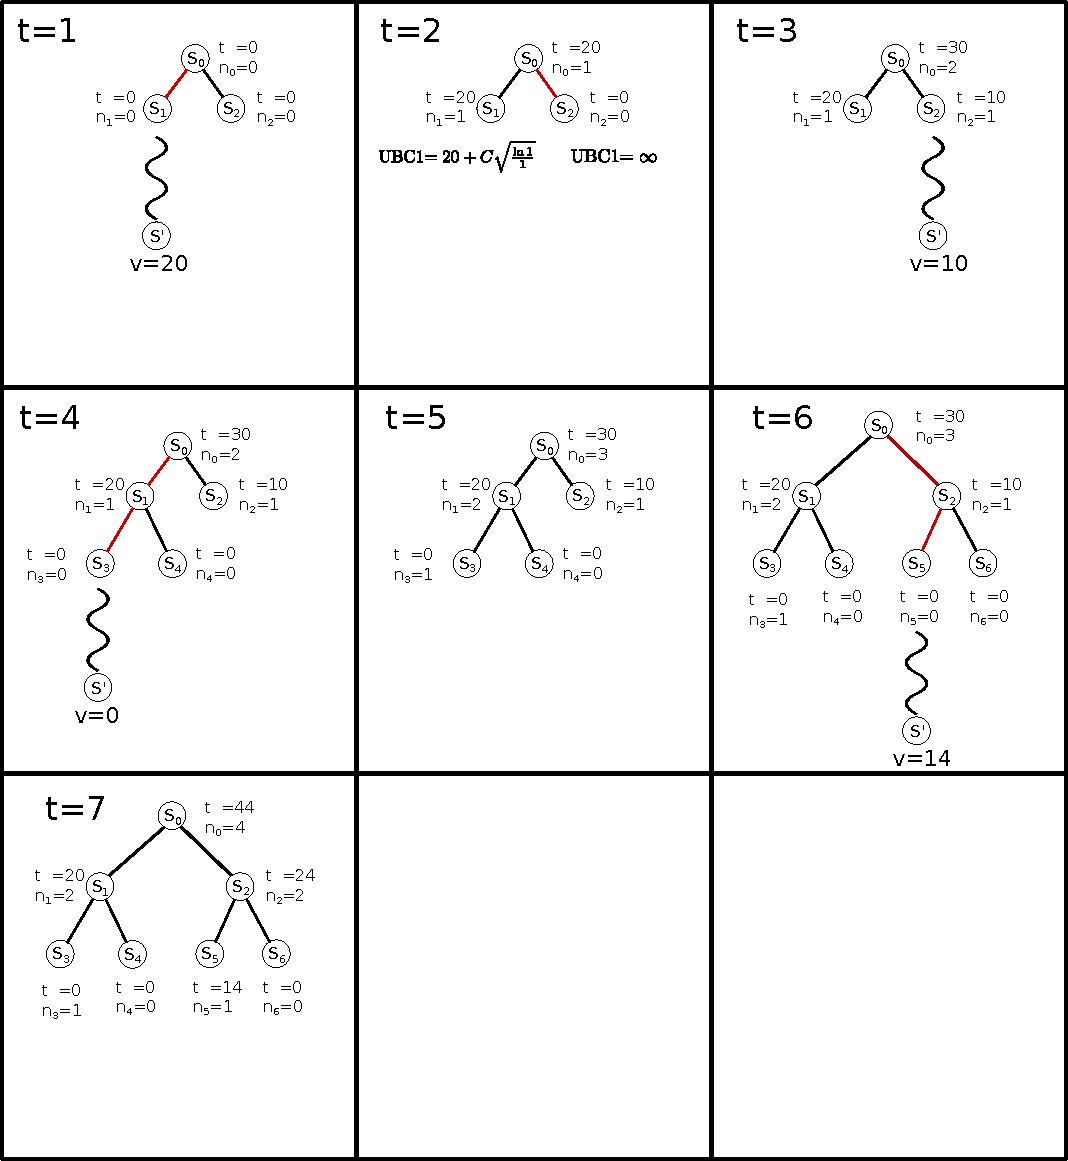
\includegraphics[scale=0.8]{./images/search_alg/mcts.pdf}
	\caption{MCTS example}
	\label{fig:mcts}
\end{figure}


\section{Uniform Cost Search}

You have three goal states, $G_1, G_2$, $G_3$. Your goal is to reach one of them. UCS is cheapest first search algorithm.

\begin{figure}[h]
	\centering
	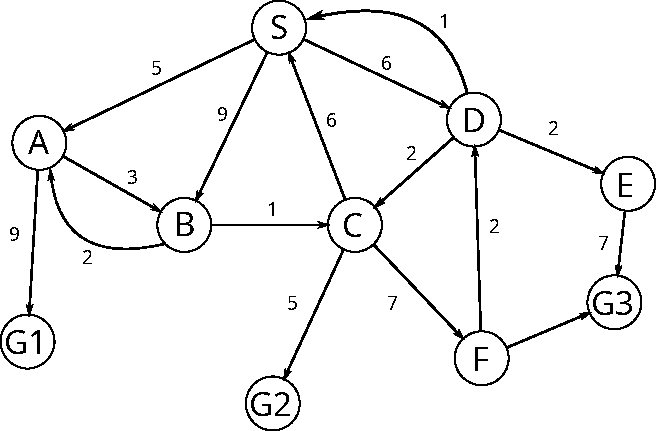
\includegraphics[scale=0.8]{./images/search_alg/uniform_sample_graph.pdf}
\end{figure}

\begin{figure}[h]
	\centering
	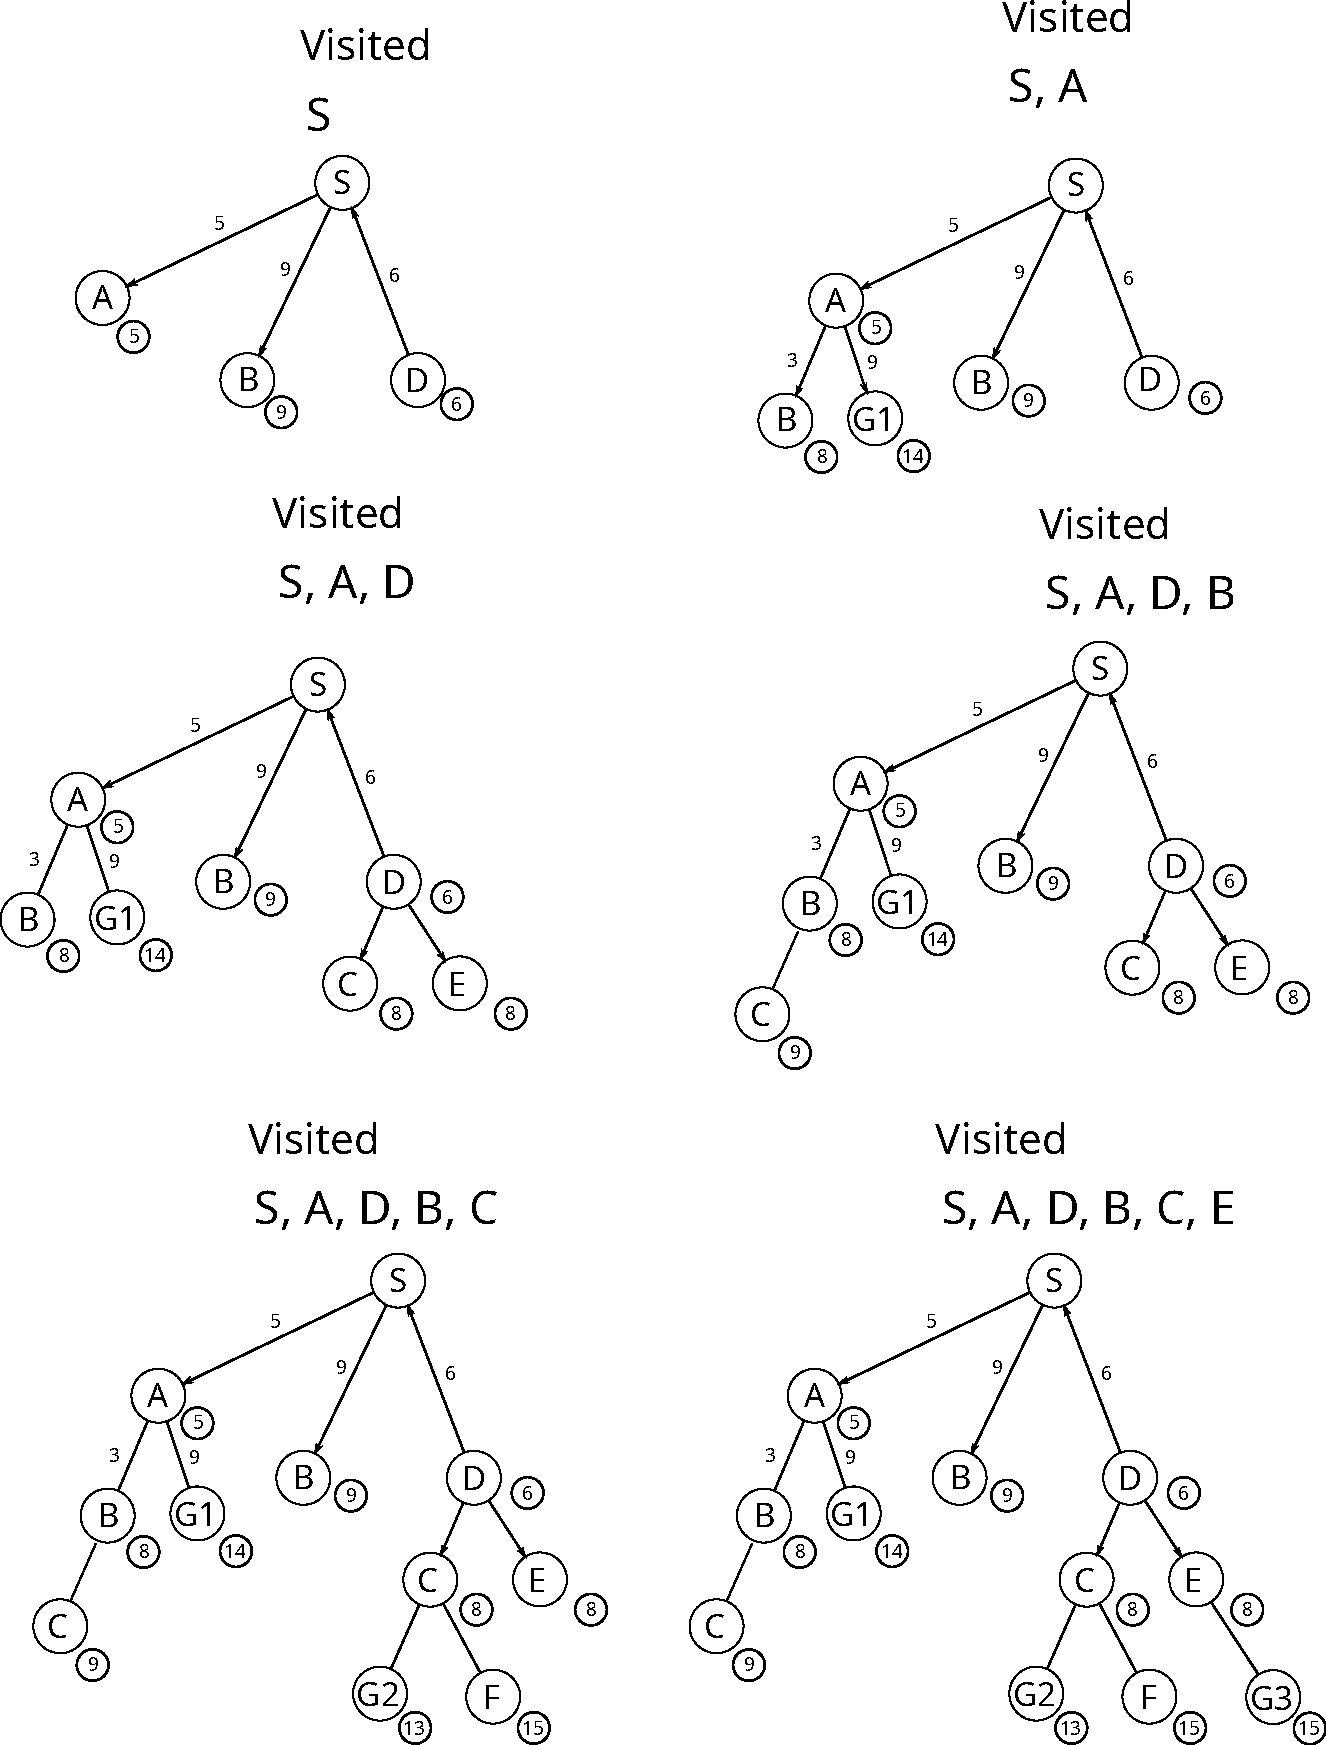
\includegraphics[scale=0.6]{./images/search_alg/uniform_cost_search.pdf}
\end{figure}

\newpage
\section{$A^*$ Search}
$A^*$ search algorithms is a variant of Dijkstra's algorithm, which incorporate additional \textit{heuristic} information about a graph. Unlike the Dijkstra's algorithm, you can specify a target node that you are interested in so that you don't have to compute all paths. 

In addition, the $A^*$ algorithm is often preferred over Dijkstra's algorithm in scenarios where the cost of reaching a goal from a particular node is not only determined by the actual distance traveled but also influenced by a heuristic estimation of the remaining distance to the goal. 

As I said, it exploits heuristics (or estimates). For instance, if we want to get a shortest path to a certain location in a map, then a very reasonable choice is to measure a distance roughly by using Euclidean distance. In \Cref{fig:astar_start}, we first initialize each node in the graph with our estimates. 

\begin{figure}[h]
	\centering
	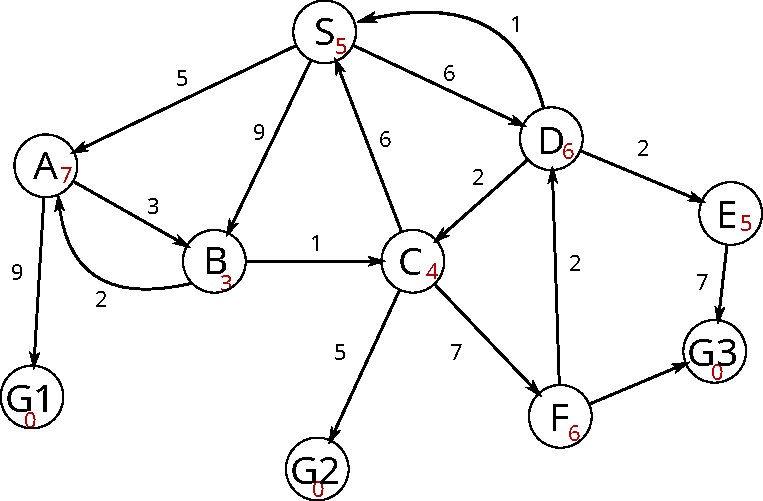
\includegraphics[scale=0.73]{./images/search_alg/astar_prob.pdf}
	\caption{Initialize $A^*$ search algorithm with heuristics.}
	\label{fig:astar_start}
\end{figure}

Then, we can explore as shown in \Cref{fig:astar_search}. For each visit, take a shortest path. 

\begin{figure}[h]
	\centering
	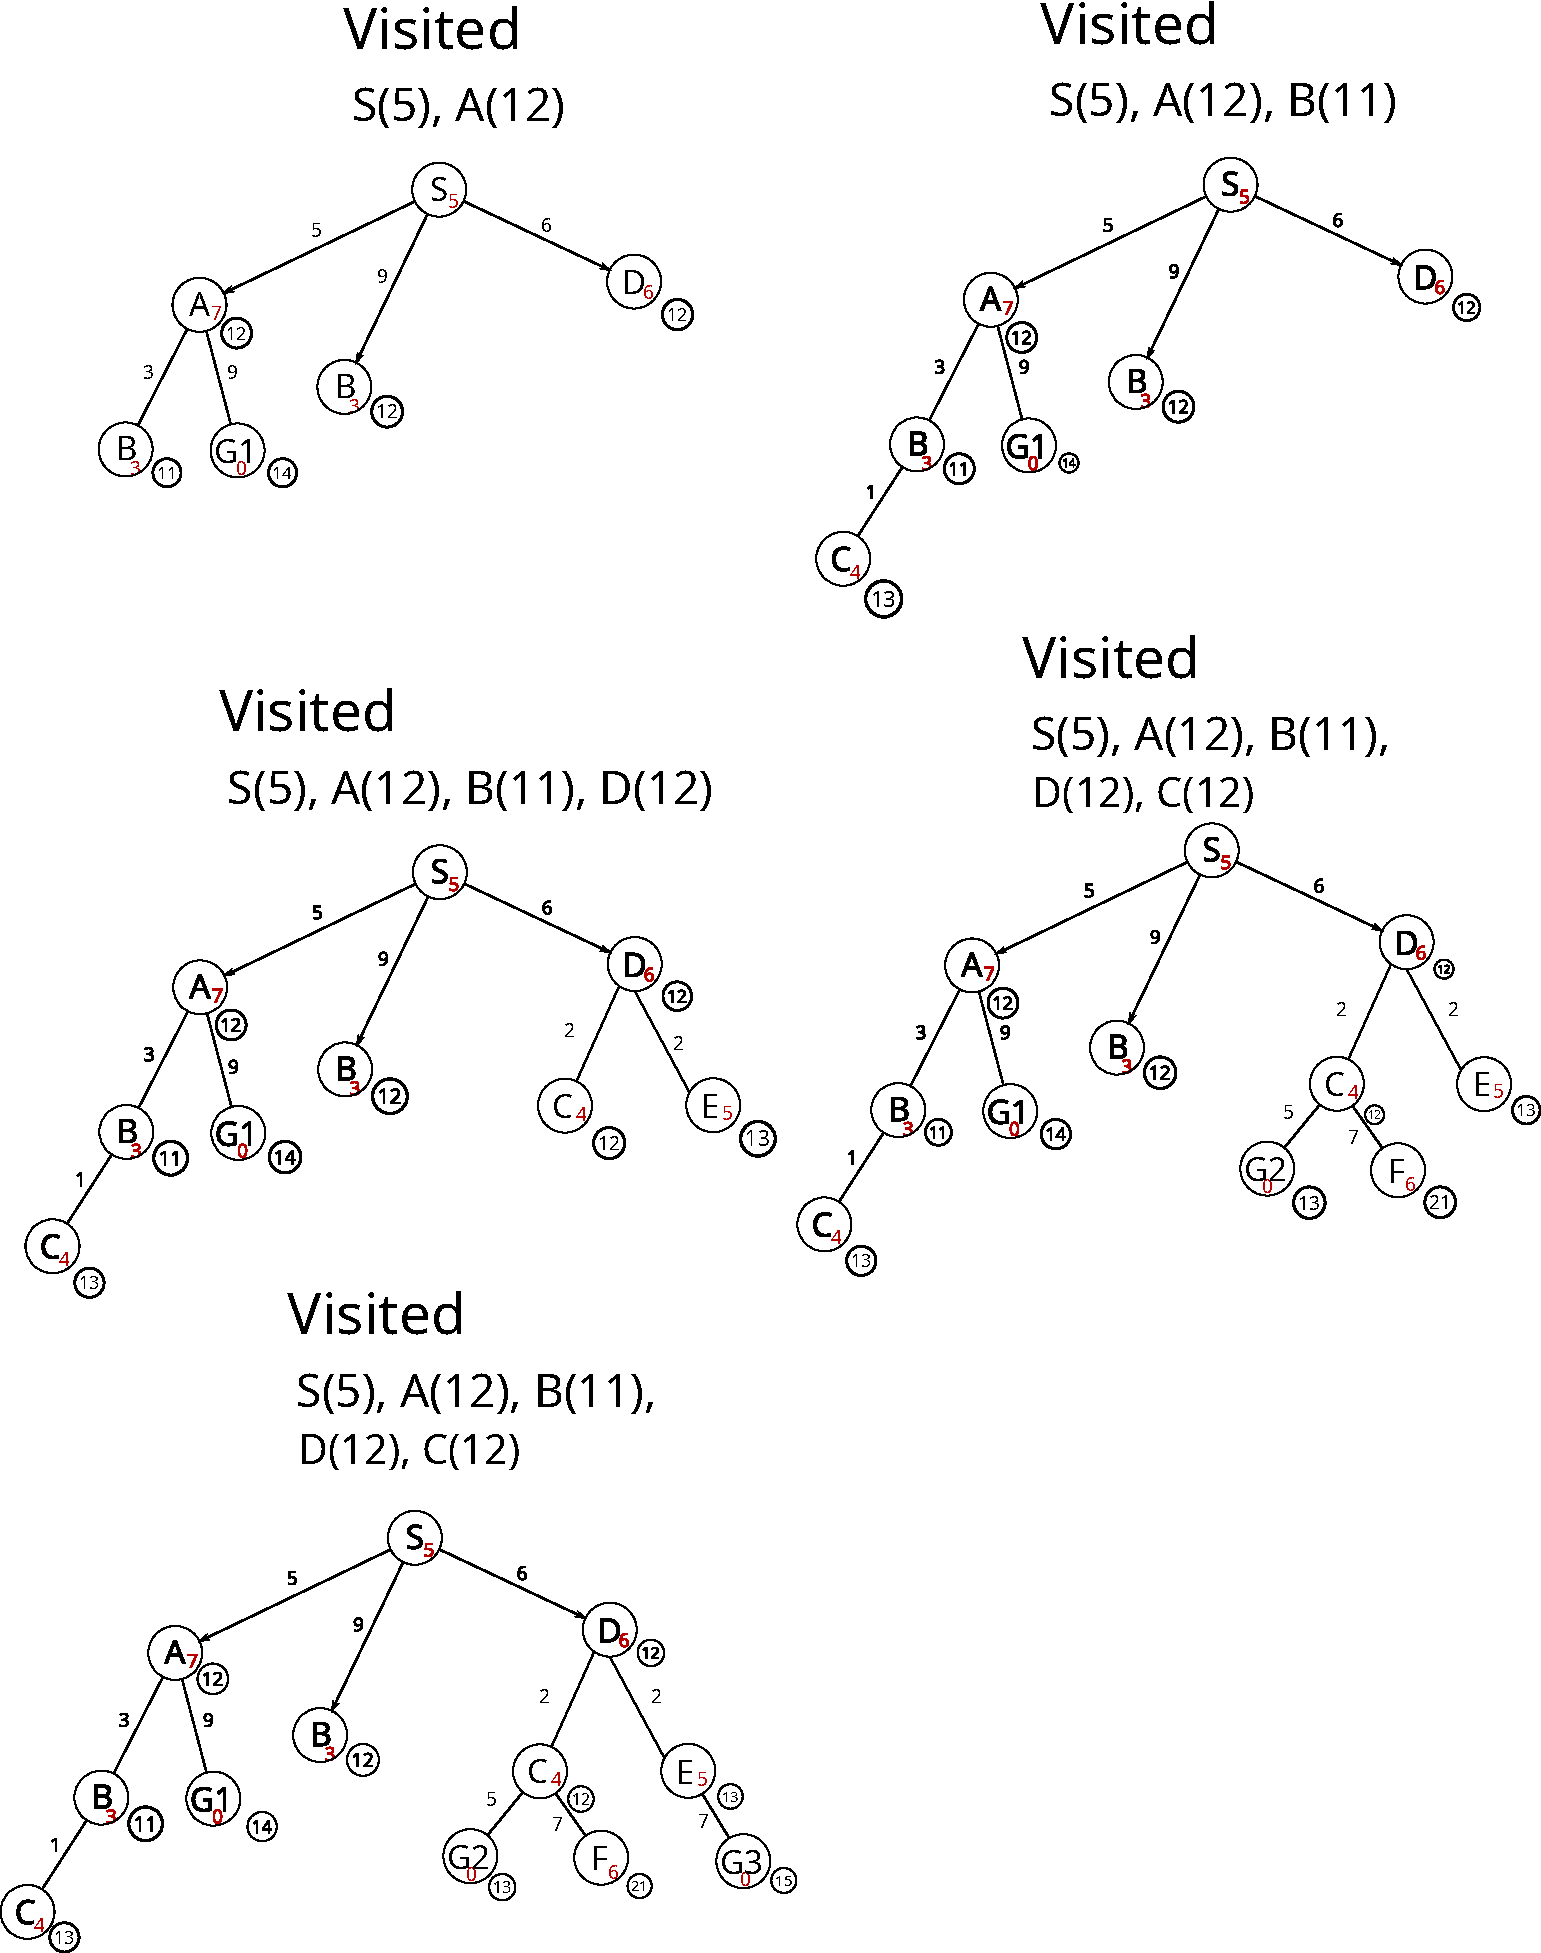
\includegraphics[scale=0.60]{./images/search_alg/astar_search.pdf}
	\label{fig:astar_search}
\end{figure}

Each number next to the nodes is called $A^*$ score, which is an estimate of cost to get to one of states. 

Note that $A^*$ algorithm is typically explained with open set and closed sets, which are just sets for nodes to be evaluated and visited. 

Open Set and Closed Set:
\begin{itemize}
	\item Open set contains nodes that need to be evaluated, 
	\item Closed set contains nodes that have already been evaluated.
\end{itemize}


\backmatter
% bibliography, glossary and index would go here.

%\nocite{*}
\bibliographystyle{unsrt}
\bibliography{references}

\appendix
\renewcommand{\thesection}{\Alph{section}.\arabic{section}}
\setcounter{section}{0}

\begin{appendices}
\chapter{Appendix}

\section{Bellman Equation}
\label{appendix:bellman_equation}

\textit{Bellman equation} can be derived as follows:

\begin{align*}
	v_\pi(s) &= \mathbb{E}_{\pi}[G_t|S_t = s]\\ 
	&= \mathbb{E}_{\pi}[R_{t+1}+\gamma G_{t+1}|S_t = s]\\ 
	&= \mathbb{E}_{\pi}[R_{t+1}|S_t = s] + \mathbb{E}_{\pi}[\gamma G_{t+1}|S_t = s], \quad \text{By Linearity of Expectation.}\\
	&= \sum_{r_{t+1}}r_{t+1} P(R_{t+1}|S_t = s) + \mathbb{E}_{\pi}[\gamma G_{t+1}|S_t = s]\\
	&= \sum_{r_{t+1}}r_{t+1} \sum_a P(R_{t+1}|S_t = s, A_t=a)P(A_t=a|S_t=s) + \mathbb{E}_{\pi}[\gamma G_{t+1}|S_t = s]\\
	&=\sum_a \sum_{r_{t+1}}r_{t+1} \sum_{s'}  P(R_{t+1}, S_{t+1}=s'|S_t = s, A_t=a)P(A_t=a|S_t=s) + \mathbb{E}_{\pi}[\gamma G_{t+1}|S_t = s]\\
&=\sum_a \sum_{r}r \sum_{s'} P(s',r|s, a)\pi(a|s) + \mathbb{E}_{\pi}[\gamma G_{t+1}|S_t = s]\\
&=\sum_a \sum_{s'} \sum_{r}r P(s',r|s, a)\pi(a|s) + \mathbb{E}_{\pi}[\gamma G_{t+1}|S_t = s]\\
&=\sum_a \sum_{s'} \mathcal{P}_{ss'}^a\mathcal{R}_{ss'}^a \pi(a|s)+ \gamma \mathbb{E}_{\pi}[ G_{t+1}|S_t = s]\\
&=\sum_a \sum_{s'}\mathcal{P}_{ss'}^a\mathcal{R}_{ss'}^a \pi(a|s) + \gamma \sum_{a}\mathbb{E}_{\pi}[ G_{t+1}|S_t = s, A_{t}=a]P(A_{t}|S_{t})\\
&=\sum_a \pi(a|s) \Bigg[\sum_{s'} \mathcal{P}_{ss'}^a\mathcal{R}_{ss'}^a + \gamma \mathbb{E}_{\pi}[ G_{t+1}|S_t = s, A_{t}=a]\Bigg]\\
&=\sum_a \pi(a|s)\Bigg[\sum_{s'} \mathcal{P}_{ss'}^a\mathcal{R}_{ss'}^a + \gamma \sum_{g_{t+1}}g_{t+1}P( G_{t+1}|S_t = s, A_{t}=a)\Bigg]\\
&=\sum_a \pi(a|s) \Bigg[\sum_{s'} \mathcal{P}_{ss'}^a\mathcal{R}_{ss'}^a + \gamma \sum_{g_{t+1}}g_{t+1}\frac{P( G_{t+1},S_t = s, A_{t}=a)}{P(S_t = s, A_{t}=a)}\Bigg]\\
&=\sum_a \pi(a|s)\Bigg[\sum_{s'} \mathcal{P}_{ss'}^a\mathcal{R}_{ss'}^a + \gamma \sum_{g_{t+1}}g_{t+1}\frac{\sum_{s'}P( G_{t+1},S_t = s, S_{t+1}=s', A_{t}=a)}{P(S_t = s, A_{t}=a)}\Bigg]\\
&=\sum_a \pi(a|s)\Bigg[\sum_{s'} \mathcal{P}_{ss'}^a\mathcal{R}_{ss'}^a + \gamma \sum_{g_{t+1}}g_{t+1}\frac{\sum_{s'}P( G_{t+1}|s, s', a)P(s, s', a)}{P(s, a)}\Bigg]\\
&=\sum_a \pi(a|s)\Bigg[\sum_{s'} \mathcal{P}_{ss'}^a\mathcal{R}_{ss'}^a + \gamma \sum_{g_{t+1}}g_{t+1}\sum_{s'}P( G_{t+1}|s, s', a)P(s'| s, a)\Bigg]\\
&=\sum_a \pi(a|s)\Bigg[\sum_{s'} \mathcal{P}_{ss'}^a\mathcal{R}_{ss'}^a + \gamma \sum_{s'}P(s'| s, a)\sum_{g_{t+1}}g_{t+1}P( G_{t+1}|s')\Bigg] \quad \textrm{by Markov Property}\\
&=\sum_a \pi(a|s)\Bigg[\sum_{s'} \mathcal{P}_{ss'}^a\mathcal{R}_{ss'}^a + \gamma \sum_{s'}\mathcal{P}_{ss'}^a v_\pi(s')\Bigg] \\
&=\sum_a \pi(a|s)\sum_{s'}\mathcal{P}_{ss'}^a\Bigg[\mathcal{R}_{ss'}^a + \gamma  v_\pi(s')\Bigg] \\
&=\sum_a \pi(a|s)\sum_{r,s'}p(s',r|s,a)\Big[r + \gamma  v_\pi(s')\Big] 
\end{align*}

Or simply, 
\begin{align*}
	v_\pi(s) &= \sum_a \pi(a|s)q(s,a)\\
	&=\sum_a \pi(a|s)\sum_{r,s'}p(s',r|s,a)\Big[r + \gamma  v_\pi(s')\Big] 
\end{align*}
%The expectation here describes what we expect the return to be if we continue from state s following policy $\pi$. The expectation can be written explicitly by summing over all possible actions and all possible returned states. The next two equations can help us make the next step.

\href{https://stats.stackexchange.com/questions/243384/deriving-bellmans-equation-in-reinforcement-learning}{Reference}

Similarly,
\begin{eqnarray*}
q_\pi(s,a) &=& \mathbb{E}_\pi[G_t|S_t=s,A_t=a]\\
&=&\mathbb{E}_\pi[R_{t+1} + \gamma G_{t+1}|S_t=s,A_t=a]\\
&=&\mathbb{E}_\pi[R_{t+1}|S_t=s,A_t=a] + \gamma\mathbb{E}_\pi[G_{t+1}|S_t=s,A_t=a]\\
&=&\sum_r rp(r|s,a) + \gamma\mathbb{E}_\pi[G_{t+1}|S_t=s,A_t=a]\\
&=&\sum_r r\sum_{s'}p(s',r|s,a) + \gamma\mathbb{E}_\pi[G_{t+1}|S_t=s,A_t=a]\\
&=&\sum_{s',r}rp(s',r|s,a) + \gamma\mathbb{E}[\mathbb{E}_\pi[G_{t+1}|S_t=s,A_t=a,R_{t+1},S_{t+1}]] \quad \text{By Law of Total Expectation.}\\
&=&\sum_{s',r} rp(s',r|s,a) + \gamma\sum_{s',r}\mathbb{E}_\pi[G_{t+1}|S_t=s,A_t=a,R_{t+1}=r,S_{t+1}=s']p(s',r|s,a)\\
&=&\sum_{s',r} p(s',r|s,a)[r + \gamma\mathbb{E}_\pi[G_{t+1}|S_t=s,A_t=a,R_{t+1}=r,S_{t+1}=s']\\
	&=&\sum_{s',r} p(s',r|s,a)[r + \gamma\mathbb{E}_\pi[G_{t+1}|S_{t+1}=s'] \quad \text{By Markov Property.}\\
&=&\sum_{s',r} p(s',r|s,a)[r + \gamma v_\pi(s')]\\
\end{eqnarray*}

\section{Importance Sampling}
You have two distributions, P(A) and P(B), and you have a sequence sampled from A. You can estimate an expectation of A, 

$$E[A] = \sum p(a)h(a).$$

Can we use the above equation for estimating an expectation of B? Yes.

$$E[B] = \sum \frac{p(b)}{p(a)}h(a).$$
The ratio $\frac{p(b)}{p(a)}$ tells us how likely to observe some results under $p(b)$ compared to $p(a)$.



%\begin{align*}
%	q_\pi(s, a) &= \mathbb{E}_{\pi}[G_t|S_t = s, A_t=a]\\ 
%	&= \mathbb{E}_{\pi}[R_{t+1}+\gamma G_{t+1}|S_t = s, A_t=a]\\ 
%	&= \sum_{s'}\mathbb{E}_{\pi}[R_{t+1}+\gamma G_{t+1}|S_t = s, A_t=a, S_{t+1}=s'] P(S_{t+1}=s'|S_t=s, A_t=a)\\ 
%	&= \sum_{s'}\mathbb{E}_{\pi}[R_{t+1}|S_t = s, A_t=a, S_{t+1}=s'] \mathcal{P}_{ss'}^a + \gamma\sum_{s'}\mathbb{E}_{\pi}[G_{t+1}|S_t = s, A_t=a, S_{t+1}=s'] \mathcal{P}_{ss'}^a \\ 
%	&= \sum_{s'}\mathbb{E}_{\pi}[R_{t+1}|S_t = s, A_t=a, S_{t+1}=s'] \mathcal{P}_{ss'}^a + \gamma\sum_{s'}\mathbb{E}_{\pi}[G_{t+1}|S_{t+1}=s'] \mathcal{P}_{ss'}^a \\ 
%	&= \sum_{s'} \sum_r r p(s',r|s,a) + \gamma\sum_{s'}v_\pi(s') \mathcal{P}_{ss'}^a \\ 
%	&= \sum_{s'}\sum_r r p(s',r|s,a) + \gamma\sum_{s'}\sum_{a'}q_\pi(s',a')\pi(a'|s') \mathcal{P}_{ss'}^a
%\end{align*}
%
%\section{Laplace Approximation}
%It works well
%
%\section{Regularized Logistic Regression}
%
%\begin{align*}
%	-\log p(\boldsymbol{w}|\boldsymbol{x}) &= -\underbrace{\log p(\boldsymbol{x}|\boldsymbol{w})}_{likelihood} - \underbrace{\log p(\boldsymbol{w})}_{Prior} + \text{const.} \\
%	&= \sum\limits_j \log \left( 1 + \exp(-y_j \boldsymbol{w}^\top \boldsymbol{x}_j) \right) + \sum\limits_i \frac{q_i (w_i - m_i)^2}{2} + \text{const.}'
%\end{align*}

\section{Fisher Information}
Suppose we have a model parameterized by parameter vector $\theta$ that models a distribution $p(x;\theta)$. In frequentist statistics, the way we learn $\theta$ is to maximize the likelihood of $p(x;\theta)$. To assess the goodness of our estimate of $\theta$ we define a \textbf{score function} as follows:
\begin{align*}
	f(\theta) = \nabla_\theta \log p(x;\theta).
\end{align*}
The expected value of score function is zero. 
\begin{align*}
	\mathbb{E}_{p(x;\theta)}[f(\theta)] &= \mathbb{E}_{p(x;\theta)}[\nabla_\theta \log p(x;\theta)]\\
	&= \int p(x;\theta) \nabla_\theta \log p(x;\theta) dx\\
	&= \int p(x;\theta) \frac{\nabla_\theta p(x;\theta)}{p(x;\theta)}  dx\\
	&= 0
\end{align*}
The covariance of the score function is given by
\begin{align*}
	\textrm{Cov}[f(\theta), f(\theta)] &= \mathbb{E}_{p(x;\theta)}[(f(\theta)-0)(f(\theta)-0)^T]= \textrm{Var}[f(\theta), f(\theta)].
\end{align*}
This the definition of Fisher information and it can be written 
\begin{align*}
	F = \mathbb{E}_{p(x;\theta)}[\nabla \log p(x;\theta)\nabla \log p(x;\theta)^T].
\end{align*}
Empirically, 
\begin{align*}
	F = \frac{1}{N}\sum_{i=1}^{N}\nabla \log p(x;\theta)\nabla \log p(x;\theta)^T.
\end{align*}

\section{Score Function}
In statistics, \textit{the score (or informant) is the gradient of the log-likelihood function with respect to the parameter vector}. 
\begin{itemize}
	\item Evaluated at a particular point of the parameter vector, the score indicates the \textbf{steepness of the log-likelihood function and thereby the sensitivity to infinitesimal changes to the parameter values}.
	\item If the log-likelihood function is continuous over the parameter space, the score will \textbf{vanish at a local maximum or minimum}; this fact is used in maximum likelihood estimation to find the parameter values that maximize the likelihood function.
\end{itemize}

Since the score is a function of the observations that are subject to sampling error, it lends itself to a test statistic known as score test in which the parameter is held at a particular value. Further, the ratio of two likelihood functions evaluated at two distinct parameter values can be understood as a definite integral of the score function.[2]

\end{appendices}


\end{document}
